%%%
%%% Master document
%%% For Brush-up kursusmateriale
%%%
%%
%% Include preamble and marcos
%%
%%%
%%% Preamble
%%% 
\documentclass[12pt]{article}
%%
%% Usual stuff
%%
\usepackage[utf8]{inputenc}
\usepackage[english]{babel}
\usepackage[T1]{fontenc}
\usepackage{lmodern}
\usepackage{xcolor}
\usepackage{hyperref}
\hypersetup{%
	%pdfpagelabels=true,%
	plainpages=false,%
	pdfauthor={Author(s)},%
	pdftitle={Title},%
	pdfsubject={Subject},%
	bookmarksnumbered=true,%
	pdfstartview=FitH%
}
\usepackage[a4paper, total={6in, 10in}]{geometry}

%%
%% Math
%%
\usepackage{amsmath}
\usepackage{amssymb}
\usepackage{mathtools}
\usepackage{mathrsfs}
\usepackage{amsthm}

\usepackage{fancyhdr}
\usepackage{lastpage}


\lhead{Benjamin Støttrup \& Kasper Sørensen}
\chead{}
\rhead{}
\lfoot{}
\cfoot{Side \thepage\ af \pageref{LastPage}}
\rfoot{}

%\setlength\parindent{0pt}
\renewcommand{\c}{\cdot}
\newcommand{\R}{\mathbb{R}}
\newcommand{\abs}[1]{\vert#1\vert}
\newcommand{\norm}[1]{\Vert#1\Vert}
\newcommand{\boundellipse}[3]% center, xdim, ydim
{(#1) ellipse (#2 and #3)
}
%%
%% Document
%%


\author{Benjamin Buus Støttrup}
\begin{document}
\pagestyle{plain}
\begin{titlepage}
    \begin{center}
        \vspace*{1cm}
        \Huge
        \textbf{Opgaver og facit til Math101}

        \vspace{0.5cm}
        \large
        Udarbejdet til Math101 kurset på Aalborg Universitet i 2018.
        \vspace{1.5cm}

        af

        \vspace{1.5cm}
        \textbf{Benjamin Buus Støttrup}

        \vfill
        Senest opdateret \today
        \vspace{2cm}




    \end{center}
    \doclicenseThis
 \end{titlepage}



\pagenumbering{roman}
\tableofcontents
\chapter*{Introduktion}\normalsize
Dette dokument indeholder en formelsamling, opgaver og facit til anvendelse i kurset Math101. Math101 er et genopfriskningskursus der typisk afholdes i efterårssemestret for de førsteårsstuderende der i løbet af semestret har fundet ud af at deres matematikniveau kunne trænge til løft. Formålet med Math101 er at give deltagerene en genopfriskning af de matematiske regnefærdigheder, primært ved at de skal løse et stort antal opgaver. Math101 kurset blev revideret i 2018 i forbindelse med at Brush-up kurserne også fik en større revidering. Math101 er tiltænkt et tilbud til de studerende der ikke benyttede sig af Brush-up, men som alligevel har brug for mere matisk rutine. Indholdet i Math101 er derfor en kraftigt reduceret version af Brush-up. Selvom emnerne går igen er opgaverne forskellige.

Math 101 består af 9 korte lektioner omhandlende følgende emner 
\begin{enumerate}
    \item Brøker, Potenser, Rødder, Kvadratsætninger.
    \item Første- og andengradsligninger.
    \item Introduktion til funktioner, herunder første-og andengradspolynomier.
    \item Inverse funktioner, Logaritme- og eksponentialfunktioner samt trigonometriske funktioner.
    \item Introduktion til differentialregning.
    \item Produktregelen, kvotientregelen og kædereglen.
    \item Bestemte og ubestemte integraler.
    \item Delvis integration og integration ved substitution.
\end{enumerate}
En lektion består typisk af en kort gennemgang af lektionens emne ud fra slides samt regning af opgaver. Alle andre opgaver bør løses uden brug af lommeregner o.l.\ elektroniske hjælpemidler. \emph{Har man ikke tænkt sig at regne i hånden kan man lige så godt lade være med at regne opgaverne!}. Bagerst i dette dokument findes en liste med svar til opgaverne. Nogle af svarene er med uddybende forklaringer, og det er ikke alle spørgsmål som kun har en løsning.


\addcontentsline{toc}{chapter}{Introduktion}
%%
%% Include Sections
%%
\pagenumbering{arabic}
\pagestyle{fancy}
\chapter{Formelsamling}
Nedenfor findes en formelsamling der dækker de emner der gennemgås i dette dokument. Formålet med formelsamlingen er at gøre det nemmere for læseren at løse opgaverne uden at skulle bladre alt for meget i dokumentet. Formelsamlingen er meget kompakt, og er derfor også velegnet til at printe og medbringe til skriftlige eksamener o.l.\ hvor det er godt at have et kompakt opslagsværk over de mest almindelige formler.
{ \newgeometry{top=5mm,bottom=5mm,left=5mm,right=5mm}
    \fontsize{8pt}{0.5pt}\selectfont
    \setlength{\abovedisplayskip}{1pt}
    \setlength{\belowdisplayskip}{1pt}
    \pagestyle{empty}
    \setlength{\parindent}{0pt}
    \small
    \begin{multicols*}{3}
        \addtocontents{toc}{\protect\setcounter{tocdepth}{0}}
        \section{Fractions}
Fractions are numbers on the form
\begin{align*}
\frac{a}{b},
\end{align*}
where $a,b$ are numbers with $b\neq 0$. $a$ is called the \emph{numerator} and $b$ is called the \emph{denominator}.
\subsection{Rules}
We have that
\begin{align*}
\frac{a}{c}\pm\frac{b}{c}&=\frac{a\pm b}{c},&&\frac{a}{b}\frac{c}{d}=\frac{ac}{bd},&&\frac{\frac{a}{b}}{\frac{c}{d}}=\frac{ad}{bc},\\
a\frac{b}{c}&=\frac{ab}{c},&&\frac{\frac{a}{b}}{c}=\frac{a}{bc},&&\frac{a}{\frac{b}{c}}=\frac{ac}{b}.
\end{align*}
\subsection{Reducing Fractions}
Common factors can be reduced:
\begin{align*}
\frac{a}{b}=\frac{ac}{bc}
\end{align*}

\section{Powers}
Powers are numbers on the form
\begin{align*}
x^a.
\end{align*}
$x$ is the \emph{base} and $a$ is the \emph{exponent}.
\subsection{Rules}
We have that
\begin{align*}
x^ax^b=x^{a+b},&& \frac{x^a}{x^b}=x^{a-b},&&(xy)^a=x^ay^a,\\
\Big(\frac{x}{y}\Big)^a=\frac{x^a}{y^a},&&(x^a)^b=x^{ab},&& x^{-a}=\frac{1}{x^a}.
\end{align*}

\section{Roots}
If $x\geq 0$ and $n\in \Z_+$ then there exists a number $\sqrt[n]{x}>0$ such that
\begin{align*}
(\sqrt[n]{x})^n=x.
\end{align*}
Note that $\sqrt[n]{x}=x^{\frac{1}{n}}$.
\subsection{Rules}
We ave that
\begin{align*}
\sqrt[n]{x}=x^{\frac{1}{n}},&& \sqrt[n]{x^m}=x^{\frac{m}{n}}=(\sqrt[n]{x})^m,\\
\sqrt[n]{xy}=\sqrt[n]{x}\sqrt[n]{y},&& \sqrt[n]{\frac{x}{y}}=\frac{\sqrt[n]{x}}{\sqrt[n]{y}}.
\end{align*}

\section{Squared Sum}
We have that
\begin{align*}
(a+b)^2&=a^2+b^2+2ab\\
(a-b)^2&=a^2+b^2-2ab\\
(a+b)(a-b)&=a^2-b^2.
\end{align*}
        \section{Equations}
Equations can be reduced with the following rules:
\begin{enumerate}
	\item You can add/subtract with the same number on both sides of an equation.
	\item You can multiply/divide with the same number (except 0) on both sides of an equation.
\end{enumerate}
\subsection{Second Order Equations}
Second order equations are on the form
\begin{align}\label{eq:lig1}
ax^2+bx+c=0,
\end{align}
The solutions to~\eqref{eq:lig1} are
\begin{align*}
x=\frac{-b\pm \sqrt{b^2-4ac}}{2a}.
\end{align*}
\subsection{Factorization}
If $ax^2+bx+c=0$ has roots $r_1$ and $r_2$ then.
\begin{align*}
ax^2+bx+c=a(x-r_1)(x-r_2).
\end{align*}
        \section{Funktioner}
En funktion $f\colon X\to Y$ tildeler alle $x\in X$ \emph{præcis ét} element $ f(x) \in Y$.

\subsection{Sammensatte funktioner}
Hvis $f\colon X\to Y$ og $g\colon Y\to Z$ defineres sammensætningen $g\circ f\colon X\to Z$ ved $(g\circ f)(x)=g(f(x))$. $f$ er den \emph{indre funktion}, $g$ er den \emph{ydre funktion}
\begin{center}
	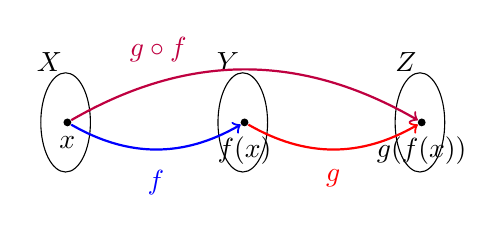
\begin{tikzpicture}[scale=0.45]
		\draw \boundellipse{0,0}{0.7}{1.4};
		\draw\boundellipse{5,0}{0.7}{1.4};
		\draw\boundellipse{10,0}{0.7}{1.4};
		\node at (0.45,1.7) [label=left:$X$]{};
		\node at (5.45,1.7) [label=left:$Y$]{}; 
		\node at (10.45,1.7) [label=left:$Z$]{}; 
		\node[circle, fill,inner sep=1pt] (x) at (0.05,0) [label=below:$x$]{};
		\node[circle, fill,inner sep=1pt] (fx) at (5.05,0) [label=below:$f(x)$]{};
		\node[circle, fill,inner sep=1pt] (gfx) at (10.05,0) [label=below:$g(f(x))$]{};
		\draw[thick,->,blue] (x) to [bend right] node[pos=0.5, label=below:$f$] {} (fx) ;
		\draw[thick,->,red] (fx) to [bend right] node[pos=0.5, label=below:$g$] {} (gfx) ;
		\draw[thick,->,purple] (x) to [bend left] node[pos=0.25, label=above:$g\circ f$] {} (gfx) ;
\end{tikzpicture}%
\end{center}
\subsection{Inverse funktioner}
To funktioner $f\colon X\to Y$ og $g\colon Y\to X$ er hinandens \emph{inverse} hvis
\begin{align*}
f(g(y))=y,\quad \textup{og}\quad g(f(x))=x 
\end{align*}
for alle $x$ i $X$ og $y$ i $Y$.

\begin{center}
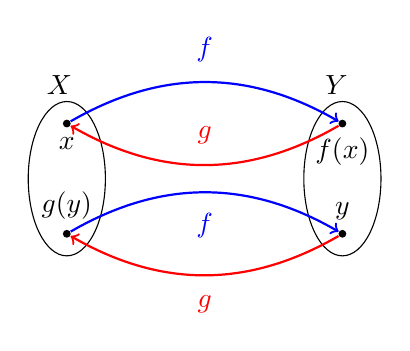
\begin{tikzpicture}[scale=0.7]
\draw \boundellipse{0,0}{0.7}{1.4};
\draw \boundellipse{5,0}{0.7}{1.4};
\node at (0.45,1.7) [label=left:$X$]{};
\node at (5.45,1.7) [label=left:$Y$]{}; 
\node[circle,fill,inner sep=1pt] (x) at (0,1) [label=below:$x$] {};
\node[circle,fill,inner sep=1pt] (gy) at (0,-1) [label=above:$g(y)$] {};
\node[circle,fill,inner sep=1pt] (fx) at (5,1) [label=below:$f(x)$] {};
\node[circle,fill,inner sep=1pt] (y) at (5,-1) [label=above:$y$] {};
\draw[thick,->,blue] (x) to[bend left]node[pos =0.5, label=above:$f$] {} (fx);
\draw[thick,->,red] (fx) to[bend left] node[pos =0.5, label=above:$g$] {} (x);
\draw[thick,->,red] (y) to[bend left]node[pos =0.5, label=below: $g$] {} (gy);
\draw[thick,->,blue] (gy) to[bend left]node[pos =0.5, label=below: $f$] {} (y);
\end{tikzpicture}%
\end{center}

\subsection{Polynomier}
Et førstegradspolynomium har forskrift:
\begin{align*}
f(x)=ax+b.
\end{align*}
Et andengradspolynomium har forskrift:
\begin{align*}
f(x)=ax^2+bx+c.
\end{align*}
\subsection{Logaritmer og eksponentialfunktioner}
\emph{Logaritmen med grundtal $a$}, $\log_a\colon ]0,\infty[\to \R$ er invers til eksponentialfunkionen $f_a(x)=a^x$ ($a>0$, $a\neq 1$). Der gælder at
\begin{align*}
\log_a(a^x)=x\quad \textup{og} \quad a^{\log_a(y)}=y
\end{align*}
og vi har
\begin{align*}
\ln x=\log_e x,&& \log x=\log_{10} x
\end{align*}
\subsection{Regneregler}
Der gælder
\begin{align*}
\log_a(xy)&=\log_a(x)+\log_a(y),\\\log_a\Big(\frac{x}{y}\Big)&=\log_a(x)-\log_a(y),\\ \log_a(x^r)&=r\log_a(x).
\end{align*}
\section{Trigonometriske funktioner}
De trigonometriske funkioner er defineret ud fra enhedscirklen:
\begin{center}
	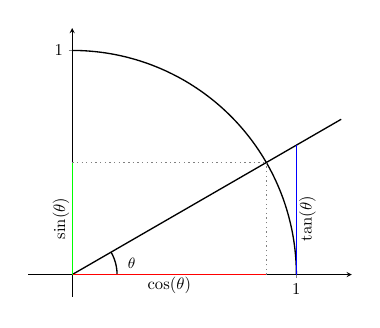
\begin{tikzpicture}[scale=0.6]
	\begin{axis}[xmin=-0.05,xmax=1.1,ymin=-0.1,ymax=1.1,axis x line=center,
	axis y line=center, axis equal, xtick={0,1},ytick={0,1}]
	%PERMANENT STUFF
	\addplot[domain=0:pi/2,thick, samples=100] ({cos(deg(x))},{sin(deg(x))});
	\addplot[domain=0:sqrt(3)/2,thick] {1/sqrt(3)*x};
	\addplot[domain=0:pi/6,thick,samples=100] ({0.2*cos(deg(x))},{0.2*sin(deg(x))}) node[label=right:{\small$\theta$},pos=0.5] {};
	%cos
	\addplot[dotted,gray,thick] coordinates {(sqrt(3)/2,0) (sqrt(3)/2, 1/2)};
	\node at (axis cs: {sqrt(3)/4},-0.05) {$\cos(\theta)$};
	\addplot[thick,red,domain=0:sqrt(3)/2] {0};
	%sin
	\node at (axis cs: -0.05,1/4) {\rotatebox{90}{$\sin(\theta)$}};
	\addplot[dotted, gray,thick,domain=0:sqrt(3)/2] {1/2};	
	\addplot[thick,green]  coordinates { (0,0) (0,1/2)};
	%tan
	\addplot[thick,domain=sqrt(3)/2:1.2] {1/sqrt(3)*x};
	\node at (axis cs: 1.05,1/4) {\rotatebox{90}{$\tan(\theta)$}};
	\addplot[blue,thick] coordinates {(1,0) (1, 1/sqrt(3)};
	\end{axis}
	\end{tikzpicture}%
\end{center}
Der gælder at
\begin{center}
\begin{tabular}{@{} lccccc @{}}
	\toprule 
	$\theta$			& 0			&$ \frac{\pi}{6} $  		&$ \frac{\pi}{4} $ 		&$ \frac{\pi}{3}$ 			&$ \frac{\pi}{2} $		\\ \midrule
	$\sin \theta$		&0			&$ \frac{1}{2} $			&$ \frac{\sqrt{2}}{2} $	& $ \frac{\sqrt{3}}{2} $ 	& 1						\\ \midrule
	$\cos \theta$		&1			&$\frac{\sqrt{3}}{2}$		&$\frac{\sqrt{2}}{2}$	& $\frac{1}{2}$				&0	\\ \midrule
	$\tan \theta$		&0			&$\frac{1}{\sqrt{3}}$		&$1$					& $ \sqrt{3} $				&-		\\ \midrule
\end{tabular}
\end{center}
samt $ \tan(\theta)=\frac{\sin(\theta)}{\cos(\theta)}$.





%\begin{tabular}{@{} lccc @{}}
%	\toprule 
%	$\theta$			& $\sin \theta$			& $\cos \theta$ 		& $\tan \theta$ 		\\ \midrule
%	0					&0						&1						&0						\\ \midrule
%	$ \frac{\pi}{6} $	&$\frac{1}{2}$			&$\frac{\sqrt{3}}{2}$	&$\frac{1}{\sqrt{3}}$	\\ \midrule
%	$ \frac{\pi}{4} $	&$\frac{\sqrt{2}}{2}$	&$\frac{\sqrt{2}}{2}$	&$1$					\\ \midrule
%	$ \frac{\pi}{3} $	&$\frac{\sqrt{3}}{2}$	&$\frac{1}{2}$			&$\sqrt{3}$				\\ \midrule
%	$ \frac{\pi}{2} $	&1						&0						&						\\ \bottomrule  
%\end{tabular}


















        \section{Derivatives}
The derivative of $f$ is denoted $f'=\frac{d}{dx}f=\frac{df}{dx}$.

\textcolor{white}{hemmelig tekst}

\subsection{Rules}
We have that
\begin{center}
		\begin{tabular}{@{}l l@{}}
		$f(x)$      & $f'(x)$  				\\ \toprule
		$c$			& $0$ 					\\ \midrule
		$x$			& $1$					\\ \midrule
		$x^n$  		& $nx^{n-1}$			\\ \midrule
		$e^x$  		& $e^x$					\\ \midrule
		$e^{cx}$  	& $ce^{cx}$				\\ \midrule
		$a^x$  		& $a^x\ln a $			\\ \midrule
		$\ln x$ 	& $\frac{1}{x}$			\\ \midrule
		$\cos x$  	& $-\sin x$				\\ \midrule
		$\sin x$  	& $\cos x$				\\ \midrule
		$\tan x$ 	& $1+\tan^2(x)$		\\ \bottomrule  
	\end{tabular}
\end{center}
\subsection{General Rules}
We have that
\begin{align*}
&(cf)'(x)=cf'(x)\\
&(f\pm g)'(x)=f'(x)\pm g'(x)\\
&(fg)'(x)=f'(x)g(x)+f(x)g'(x)\\
&\Big(\frac{f}{g}\Big)'(x)=\frac{f'(x)g(x)-f(x)g'(x)}{g^2(x)}\\
&\frac{d}{dx}f(g(x))=f'(g(x))g'(x).
\end{align*}
The last formula is also called the \emph{chain rule}.
        \section{Ubestemte integraler}
En funktion $f$ har \emph{stamfunktion} $F$ hvis
\begin{align*}
F'(x)=f(x).
\end{align*}
Det ubestemte integral af $f$ defineres til
\begin{align*}
\int f(x)\, dx =F(x)+k,
\end{align*}
hvor $F$ er en stamfunktion til $f$ og $k\in \R$.
\subsection{Generelle regneregler}
\begin{align*}
&\int cf(x) \, d x=c\int f(x)\, dx\\
&\int f(x)\pm g(x) \, d x=\int f(x)\, dx\pm \int g(x) \, dx.\\
&\int f(x)g(x)\, dx=f(x)G(x)-\int f'(x)G(x)\, dx\\
&\int f(g(x))g'(x)\, dx =F(g(x))+k.
\end{align*}
Den 3. regel kaldes \emph{delvis integration} og den sidste kaldes \emph{integration ved substitution}.
\subsection{Regneregler}
Der gælder at
\begin{center}
		\begin{tabular}{@{}l l@{}}
		$f(x)$      & $\int f(x)\, dx$  				\\ \toprule
		$c$			& $cx+k$ 							\\ \midrule
		$x$			& $\frac{1}{2}x^2+k$				\\ \midrule
		$x^n$  		& $\frac{1}{n+1}x^{n+1}+k$			\\ \midrule
		$e^x$  		& $e^x+k$							\\ \midrule
		$e^{cx}$  	& $\frac{1}{c}e^{cx}+k$				\\ \midrule
		$\frac{1}{x}$ & $\ln(\vert x\vert)+k $			\\ \midrule
		$\ln x$ 	& $x\ln(x)-x+k$						\\ \midrule
		$\cos x$  	& $\sin x+k$						\\ \midrule
		$\sin x$  	& $-\cos x+k$						\\ \midrule
		$\tan x$ 	& $-\ln(\vert \cos(x)\vert)+k$		\\ \bottomrule  
	\end{tabular}
\end{center}
\subsection{Integration ved substitution}
Givet et integral på formen $\int f(g(x))g'(x)\, dx$ anvendes metoden:
\begin{enumerate}
	\item Lad $u=g(x)$.
	\item Udregn $\frac{du}{dx}$ og isoler $dx$.
	\item Substituer $g(x)$ og $dx$.
	\item Udregn integralet mht. $u$.
	\item Substituer tilbage.
\end{enumerate}
\section{Besemte integraler}
Det bestemte integral af $f$ i intervallet $[a,b]$ til
\begin{align*}
\int_a^b f(x)\, dx =[F(x)]_a^b=F(b)-F(a),
\end{align*}
hvor $F$ er en stamfunktion til $f$.
\subsection{Generelle regneregler}
\begin{align*}
&\int_a^b cf(x) \, d x=c\int_a^b f(x)\, dx\\
&\int_a^b \!\!f(x)\pm g(x) \, d x=\int_a^b\!\!f(x)\, dx\pm \int_a^b\!\! g(x) \, dx\\
&\int_a^b\!\!\! \!\!\!f(x)g(x)\, dx\!\!=\!\![f(x)G(x)]_a^b\!\!-\!\!\!\!\int_a^b\!\!\!\!\!\! f'(x)G(x)\, dx\\
%&\phantom{\int_a^b f(x)g(x)\, dx=}-\int_a^b f'(x)G(x)\, dx\\
&\int_a^b f(g(x))g'(x) \, dx=[F(x)]_{g(a)}^{g(b)}.
\end{align*}
\subsection{Integration ved substitution}
Givet et integral på formen $\int_a^b f(g(x))g'(x)\, dx$ anvendes metoden
	\begin{enumerate}
	\item Lad $u=g(x)$.
	\item Udregn $\frac{du}{dx}$ og isoler $dx$.
	\item Substituer $g(x)$, $dx$ samt grænser.
	\item Udregn integralet mht. $u$.
\end{enumerate}
        % \mysection{Differentialligninger}


\mysubsection{Løsningsformler}
\begin{center}
\begin{tabular}{@{}l l@{}}
Differentiallign.    & Fuldstændig løsn.				\\ \toprule
$f'(x)=k$				& $f(x)=kx+c$						\\ \midrule
$f'(x)=h(x)$			& $f(x)=\int h(x) \d x$				\\ \midrule
$f'(x)=kf(x)$			& $f(x)=ce^{kx}$					\\ \midrule
$f'(x)+ af(x) =b$		& $f(x)=\frac{b}{a}+ce^{-ax}$		\\ \bottomrule  
\end{tabular}
\end{center}

\mysubsection{Panserformlen}
Differentialligningen 
\begin{equation*}
f'(x)+a(x)f(x)=b(x)
\end{equation*}
har fuldstændig løsning
\begin{equation*}
f(x)=e^{-A(x)}\int b(x) e^{A(x)}dx +ce^{-A(x)},
\end{equation*}
hvor $A'(x)=a(x)$.
        % \mysection{Vektorer i planen}
En vektor $\vec{u}$ i planen skrives som $\vec{u}=[x,y]$ hvor $x,y\in \R$.
\mysubsection{Regneregler}
For $\vec{u}=[x_1,y_1]$, $\vec{v}=[x_2,y_2]$, $c\in \R$ er 
\begin{align*}
    \vec{u}\pm\vec{v}=\begin{bmatrix}
        x_1\pm x_2\\y_1\pm y_2
    \end{bmatrix}, &&\vec{u}\cdot\vec{v}=x_1x_2+y_1y_2 ,\\
    c\vec{u}=\begin{bmatrix*}
        cx_1\\cy_1
    \end{bmatrix*}, && \!\!\!\det(\vec{u},\vec{v})=x_1y_2-x_2y_1
\end{align*}
Længden af $\vec{u}$ er $\left\Vert \vec{u}\right\Vert=\sqrt{x_1^2+y_1^2}$.
\mysubsection{Vinklen mellem to vektorer}
For vinklen $\theta$ mellem $\vec{u}$, $\vec{v}$ er 
\begin{align*}
    \cos\theta=\frac{\vec{u}\cdot\vec{v}}{\left\Vert \vec{u}\right\Vert \left\Vert \vec{v}\right\Vert }, && \sin\theta=\frac{\det(\vec{u},\vec{v})}{\left\Vert \vec{u}\right\Vert \left\Vert \vec{v}\right\Vert}
\end{align*}
Yderligere gælder 
\begin{enumerate}
    \item $\vec{u}$ og $\vec{v}$ er ortogonale $\Leftrightarrow $ $\vec{u}\cdot\vec{v}=0$.
    \item $\vec{u}$ og $\vec{v}$ er parallelle $\Leftrightarrow$ $\det(\vec{u},\vec{v})=0$.
\end{enumerate}
\
\mysection{Vektorer i rummet}
En vektor $\vec{u}$ i rummet skrives som $\vec{u}=[x,y,z]$ hvor $x,y,z\in \R$.
\mysubsection{Regneregler}
For $\vec{u}=[x_1,y_1,z_1]$, $\vec{v}=[x_2,y_2,z_2]$ og $c\in \R$ gælder 
\begin{align*}
    &\vec{u}\pm\vec{v}=\begin{bmatrix}
        x_1\pm x_2\\y_1\pm y_2\\z_1\pm z_2
    \end{bmatrix}, && c\vec{u}=\begin{bmatrix*}
        cx_1\\cy_1\\c z_1
    \end{bmatrix*},\\
    &\vec{u}\cdot\vec{v}=x_1x_2+y_1y_2+z_1z_2. &&
\end{align*}
Længden af $\vec{u}$ er $\left\Vert \vec{u}\right\Vert=\sqrt{x_1^2+y_1^2+z_1^2}$. Krydsproduktet er givet ved 
\begin{equation*}
    \vec{u}\times \vec{v}=\begin{bmatrix}
        y_1z_2-z_1y_2\\ z_1x_2-x_1z_2\\x_1y_2-y_1x_2
    \end{bmatrix}
\end{equation*}
\mysubsection{Vinklen mellem to vektorer}
For vinklen $\theta$ mellem $\vec{u}$ og $\vec{v}$ gælder 
\begin{align*}
    \cos\theta=\frac{\vec{u}\cdot\vec{v}}{\left\Vert \vec{u}\right\Vert \left\Vert \vec{v}\right\Vert }, && \sin\theta=\frac{\left\Vert \vec{u}\times \vec{v}\right\Vert }{\left\Vert \vec{u}\right\Vert \left\Vert \vec{v}\right\Vert}
\end{align*}
Yderligere gælder 
\begin{enumerate}
    \item $\vec{u}$ og $\vec{v}$ er ortogonale $\Leftrightarrow$ $\vec{u}\cdot\vec{v}=0$.
    \item $\vec{u}$ og $\vec{v}$ er parallelle $\Leftrightarrow$ $\vec{u}\times\vec{v}=0$.
\end{enumerate}
\mysection{Linjer og Planer}
Planen/linjen gennem punktet med stedvektor $\vec{x}_0$ med normalvektor $\vec{n}$ beskrives ved alle vektorer $\vec{x}$ der løser ligningen
\begin{equation*}
    \vec{n}\cdot(\vec{x}-\vec{x_0})=0
\end{equation*}
En linje i rummet/planen gennem punktet med stedvektor $\vec{x}_0$ og retning $\vec{r}$ har parameterfremstilling
\begin{align*}
    \vec{x}_0+t\vec{r}, \quad t\in \R.
\end{align*}
        \phantom{asdfjæasdjfæsalkdjfælsadjfælksadjfælksadjfælkadsjfælksadjfælsakdjfælsakdjfælsakdjfælksadjfælakdsjfældsakjfæl}
        \vfill
    \end{multicols*}
    }
\restoregeometry
\addtocontents{toc}{\protect\setcounter{tocdepth}{1}}
\chapter{Opgaver}
\subsection{Opgaver}

\begin{enumerate}
\item Omskriv følgende tal til brøker hvor nævneren er 4:
\begin{align*}
2,&& \iffalse 5,&&  \frac{4}{8},&& \fi \frac{60}{24},&& \pi,&& \frac{3}{2}.% ,&& \frac{12}{16},&&30.
\end{align*}
\item Omskriv følgende tal til brøker hvor nævneren er 3:
\begin{align*}
7,&& \iffalse 3,&&\frac{2}{6},&& \fi \frac{6}{9},&&\frac{16}{12},&&4\pi.% && \frac{14}{21},&&e.
\end{align*}
\item Udregn følgende tal (forkort mest muligt):
\begin{align*}
\frac{6}{7}+\frac{8}{7},&& \frac{1}{2}+\frac{3}{4},&& \frac{1}{2}+\frac{1}{3}+\frac{1}{4},&& \frac{3}{2}-\frac{4}{8},&&-\frac{2}{3}+\frac{2}{6}.
\end{align*}
\item Udregn følgende tal (forkort mest muligt):
\begin{align*}
2\c\frac{3}{4},&&\frac{1}{8}\c \frac{2}{3},&& \frac{7}{8}\c \frac{1}{3},&& 2\c3\c \frac{1}{4}\c\frac{1}{5},&&\frac{2}{3}\c \frac{7}{3},&&\frac{3}{5}\c \frac{15}{25}.
\end{align*}
\item Udregn følgende tal (forkort mest muligt):
\begin{align*}
\frac{6}{ \frac{3}{2}},&& \frac{ \frac{2}{3}}{ \frac{4}{9}},&& \frac{ \frac{3}{2}}{6},&& \frac{ \frac{2}{7}}{ \frac{14}{49}},&& \frac{ (\frac{1}{2}:\frac{3}{4})}{ \frac{8}{15}}.
\end{align*}
\item Forkort følgende brøker mest muligt:
\begin{align*}
\frac{x^2+x}{x},&& \frac{2x+4y}{2},&& \frac{2xy+7y}{y},&&\frac{x^2y+xy}{x(x+1)},&& \frac{(x+3)^2}{2x^2+6x},&& \frac{2 (x-1)^2}{6x^2-6x}.
\end{align*}
\item Udregn følgende tal (forkort mest muligt):
\begin{align*}
\frac{3}{2}-\bigg(\frac{1}{5}\c \frac{2}{10}\bigg),&& -21\bigg( \frac{2}{3}- \frac{1}{7}\bigg),&& \frac{2}{4}\c \frac{8}{4}-\frac{3}{8},&& \frac{\frac{2}{5}}{3}-2\c \frac{2}{30},&& \frac{6}{ \frac{2}{3}} +\frac{1}{2}.
\end{align*}
\item Reducer følgende brøk mest muligt:
\begin{align*}
\frac{a-(2b-9)}{a-2b}-\frac{a-(b-5)}{a-2b}+\frac{a-(b+4)}{a-2b}.
\end{align*}
\item Indsæt det tal som mangler:
\begin{align*}
\frac{1}{2}= \frac{3}{},&& \frac{6}{7}=\frac{}{49},&& \frac{2x}{y}=\frac{2xy}{},&& \frac{ \pi}{\sqrt{2}}=\frac{}{3 \pi^2 \sqrt{2}}.
\end{align*}
\item Udregn følgende tal (forkort mest muligt):
\begin{align*}
\frac{ \frac{1}{2}+\frac{2}{5}}{1+\frac{1}{10}},&& \frac{ \frac{3}{4}+1}{ \frac{9}{8}-1},&& \frac{2}{3}\c \frac{ \frac{5}{2}-2}{ \frac{8}{3}+1}.
\end{align*}
\item Reducer følgende brøk:
\begin{align*}
\frac{4a+(2c-4b)}{a-b} - (c-2)-\frac{2c-ac+bc}{a-b}.
\end{align*}
\item Vis, at
\begin{align*}
\frac{ \frac{1}{b}+1 }{1- \frac{a}{b}}=\frac{1+b}{b-a},
\end{align*}
hvor $b\notin \{0,a\}$.
\item Vis at
\begin{align*}
\frac{ \frac{a}{b}+1}{ \frac{b}{a}+1}=\frac{a}{b},
\end{align*}
hvor $a,b\neq 0$ og $a\neq -b$. Hvorfor kræver vi at $a,b\neq 0$ samt at $a\neq -b$?
\end{enumerate}

\subsection{Opgaver}

\begin{enumerate}
\item Reducer følgende udtryk:
\begin{align*}
(x+1)^2,&& (2x-3)^2,&& (x-2)(x+2)+4,&& (3a-2b)^2+6ab.
\end{align*}
\item Forkort følgende børker
\begin{align*}
\frac{(x+3)^2}{2x^2+6x},&& \frac{4x^2-9}{4x^2+9-12x},&& \frac{2x^2+18+12x}{x^2+3x},&& \frac{(x-y)^2-y^2}{2x}.
\end{align*}
\item Følgende ligninger beskriver cirkler i planen. Angiv deres centrumskoordinater og radius.
\begin{align*}
x^2+y^2=1,&& x^2-2x+y^2+2y-23=0,&& x^2+4x+y^2=0.
\end{align*}
\item Udregn følgende tal.
\begin{align*}
99^2-101^2,&& 999^2,&& 499^2-501^2,&& 99998^2-100002^2.
\end{align*}
\item Reducer følgende udtryk
\begin{align*}
(a-2)^2-(a-2)(a+2),&& \frac{x^2-y^2}{x-y}+\frac{x^2-y^2}{x+y},&&\frac{ 4x^2+9+12x}{2x-3}-\frac{24}{2- \frac{3}{x}}.
\end{align*}
\item Følgende ligninger beskriver cirkler i planen. Angiv deres centrumskoordinater og radius.
\begin{align*}
2x^2-12x+2y^2-16y=0,&& x^2-x+y^2+y=\frac{1}{2}.
\end{align*}
\item \label{it:1} Gør rede for hvordan formlen $(a+b)^2=a^2+b^2+2ab$ kan illustreres med Figur~\ref{fig:1}.
\item \label{it:2} Gør rede for hvordan formlen $(a-b)(a+b)=a^2-b^2$ kan illustreres med Figur~\ref{fig:2}.
\item \label{it:3} Vis Pythagoras' Sætning $a^2+b^2=c^2$ ved hjælp af Figur~\ref{fig:3}.

\item \label{it:ex13} Reducer følgende udtryk:
\begin{align*}
(-a-6b)^2,&& (-4-a)(-4+a),&& \Big(x+\frac{1}{x}\Big)^2.
\end{align*}
\item Vis, at
\begin{align*}
\frac{7a +b}{4a^2-4b^2}-\frac{3}{4a+4b}-\frac{3}{4a-4b}=\frac{1}{4a-4b}.
\end{align*}

\item \label{it:4} Vis at
\begin{align*}
(a+b+c)^2= a^2+b^2+c^2+2ab+2ac+2bc.
\end{align*}
(Hint: lad $d=b+c$ og start med at betragte $(a+d)^2$.)
\item\label{it:eks21} Lad $a,b,c$ være reelle med $a\neq 0$. Bestem konstanter $d,k$ således at ligningen
\begin{align*}
ax^2+bx+c=0
\end{align*}
kan omskrives til 
\begin{align*}
(x+k)^2=\frac{d}{4a^2}.
\end{align*}
(Hint: Divider med $a$ og brug en kvadratsætning.)

\begin{figure}
\centering
\begin{tikzpicture}
\draw (0,0)--(5,0)--(5,5)--(0,5)-- cycle;
\draw[dashed] (0,4)--(5,4);
\draw[dashed] (4,0)--(4,5);
\node at (2,0) [label=below: $a$] {};
\node at (4.5,0) [label=below:$b$] {};
\node at (0,2) [label=left: $a$] {};
\node at (0,4.5) [label=left:$b$] {};
\node at (2,5) [label=above: $a$] {};
\node at (4.5,5) [label=above:$b$] {};
\node at (5,2) [label=right: $a$] {};
\node at (5,4.5) [label=right:$b$] {};
\end{tikzpicture}
\caption{Opgave~\ref{it:1}}
\label{fig:1}
\end{figure}
%
\begin{figure}
\centering
\begin{tikzpicture}
\draw (0,0)--(0,4)--(4,4)--(4,0)--cycle;
\draw[pattern=north east lines] (0,0)--(3,0)--(3,1)--(0,4)--cycle;
\draw[fill=gray] (3,1)--(0,4)--(4,4)--(4,1)--cycle;
\node at (1.5,0) [label=below: $a-b$] {};
\node at (3.5,0) [label=below:$b$] {};
\node at (0,2) [label=left: $a$] {};
\node at (2,4) [label=above: $a$] {};
\node at (4,2.5) [label=right: $a-b$] {};
\node at (4,0.5) [label=right:$b$] {};
%%%Newfig
\draw (8,0)--(11,0)--(11,5)--(8,5)--cycle;
\draw[pattern=north east lines] (8,0)--(8,4)--(11,1)--(11,0)--cycle;
\draw[fill=gray] (8,4)--(8,5)--(11,5)--(11,1)-- cycle;
\node at (9.5,0) [label=below: $a-b$] {};
\node at (8,2) [label= left: $a$] {};
\node at (8,4.5) [label= left: $b$] {};
\node at (9.5,5) [label= above: $a-b$] {};
\node at (11,3) [label= right: $a$] {};
\node at (11,0.5) [label= right: $b$] {};
\end{tikzpicture}
\caption{Opgave~\ref{it:2}}
\label{fig:2}
\end{figure}
\begin{figure}
\centering
\begin{tikzpicture}[auto]
\draw (0,0)--(0,5)--(5,5)--(5,0)--cycle;
\draw (0,3)-- node {$c$} (2,0) ;
\draw (0,3)--node {$c$} (3,5);
\draw (3,5)--node {$c$} (5,2);
\draw (2,0)-- node {$c$} (5,2);
\node at (1,0) [label=below: $a$] {};
\node at (3.5,0) [label=below: $b$] {};
\node at (0,1.5) [label=left: $b$] {};
\node at (0, 4) [label=left: $a$] {};
\node at (1.5,5) [label=above: $b$] {};
\node at (4,5) [label=above: $a$] {};
\node at (5,1)  [label= right: $a$] {};
\node at (5,3.5) [label=right: $b$] {};
\end{tikzpicture}
\caption{Opgave~\ref{it:3}}
\label{fig:3}
\end{figure}
\end{enumerate}
\subsection{Opgaver}

\begin{enumerate}
\item Udregn følgende potenser
\begin{align*}
1^{999},&&0^{123},&& 2^4,&&5^3,&& 3^4,&& 6^2.
\end{align*}
\item Udregn følgende potenser
\begin{align*}
(-3)^3,&& 6^{-2},&& \Big(\frac{1}{2}\Big)^{3},&& \Big(\frac{1}{3}\Big)^{-1},&& (-2)^4,&& 10^{-3}.
\end{align*}
\item Udregn følgende potenser
\begin{align*}
\frac{5^3}{5^2},&& \frac{2}{2^{-3}},&& 3^2\c 3^2,&& 2^{-3}(-2)^3,&& \frac{3^{12}}{3^9}.
\end{align*}
\item Antag at $0\leq x\leq1$. Bestem med udgangspunkt i \href{https://www.geogebra.org/m/Kdr3GHkr}{GeoGebra} :
\begin{enumerate}
\item Hvilke værdier af $a$ opfylder $x^a\leq x$?
\item Hvilke værdier af $a$ opfylder $x^a \geq x$?
\item Hvad sker med $x^a$ hvis $a$ vokser?
\item Hvad sker med $x^a$ hvis $a$ aftager?
\end{enumerate}
\item Antag at $x>1$. Bestem med udgangspunkt i \href{https://www.geogebra.org/m/Kdr3GHkr}{GeoGebra}:
\begin{enumerate}
\item Hvilke værdier af $a$ opfylder $x^a\leq x$?
\item Hvilke værdier af $a$ opfylder $x^a \geq x$?
\item Hvad sker med $x^a$ hvis $a$ vokser?
\item Hvad sker med $x^a$ hvis $a$ aftager?
\end{enumerate}
 
\item Reducer følgende udtryk
\begin{align*}
(2x^2)^2,&& \Big(\frac{(xy)^{3}}{x}\Big)^{-3},&& x^3\c (3x)^2x^{-4} \frac{x^0}{x^{-5}},&& \frac{(x^2)^3}{x^5}.
\end{align*}
\item Omskriv til tal på formen $2^n3^m$.
\begin{align*}
6^2,&& 3\cdot \Big(\frac{4}{3}\Big)^3,&& \frac{12^2}{2^2},&& 24\c 12^{-2}\c 6^3\c 3^{-4},&& \Big(\frac{4}{9}\Big)^{2}.
\end{align*}
\item Reducer følgende udtryk
\begin{align*}
\frac{9a^2b^5}{3(ab)^3},&& \frac{6a^3b^{-4}}{(2a^2b)^2},&& \frac{2x^{-4}y^3}{(2y^2x)^{-2}}.
\end{align*}

\item Vis at 
\begin{align*}
(a+b)^4=a^4+4a^3b+6a^2b^2+4	ab^3+b^4.
\end{align*}
(Hint: Brug at $(a+b)^4=((a+b)^2)^{2}$, samt kvadratsætningerne og Opgave~\ref{it:4} fra sidst.)
\item Reducer følgende udtryk
\begin{align*}
x^3(xy)^8y^{-4}zz^{-5},&& \frac{xz^2y^{-3}(xyz)^{-3}}{xyz^4},&& \Big(\frac{xy^4z^{-1}x^2y}{zx^5y^{2}(xy)^3}\Big)^{-2}
\end{align*}
\item Omskriv til tal på formen $\Big(\frac{1}{2}\Big)^m 3^n$.
\begin{align*}
\frac{ \Big( \frac{3}{4}\Big)^{3}2^4(3^{-2})^{3}}{3^{-3}2^{10}},&& \frac{2^3 6^3 12^3 3^{-8}}{4^2 9^3},&& \frac{(12)^{-1}\frac{3}{2^3}2^{-1}}{6^2}.
\end{align*}


\end{enumerate}

\section{Inverse funktioner, logaritme- og eksponentialfunktioner samt trigonometriske funktioner}
\begin{enumerate}
	\item Udregn følgende tal
	\begin{align*}
	3^3,&& 2^{-1}, &&\Big(\frac{1}{-1}\Big)^{3},&&\Big(\frac{1}{2}\Big)^{-3},&& 123^0.
	\end{align*}
	\item Udregn følgende tal
	\begin{align*}
	\log_2(128),&& \log_{10}(100),&& \log_5\Big(\frac{1}{25}\Big),&& \ln(e^3),&&\log_{123}(1).
	\end{align*}
	
	\item Udregn følgende tal
	\begin{align*}
	\sin(\frac{\pi}{4})+\cos(\frac{\pi}{4}),&& \tan(\frac{\pi}{3})+\cos(\frac{\pi}{6}),&& \frac{\sin(\frac{\pi}{6})+\cos(\frac{\pi}{3})}{\sin(\frac{2\pi}{3})}.
	\end{align*}
	

	\item Udregn følgende tal
	\begin{align*}
	\log_{10}(4)+\log_{10}(250),&&\log_{10}(25)-\log_{10}(5)+\log_{10}(2),&& \log_3(54)+\log_3\Big(\frac{1}{2}\Big)
	\end{align*}
	
	\item Udregn følgende
	\begin{align*}
	\cos(-\frac{5\pi}{4}),&& \sin(\frac{5\pi}{3}),&&\tan(-\frac{5\pi}{4}),&& \cos(\frac{8\pi}{3}).
	\end{align*}
	
	
	\item Reducer følgende
	\begin{align*}
	\ln(\sqrt{2})+\ln(2),&& \log_{10}(5^{3/2})+\frac{1}{2}\log_{10}(5)+\log_{10}(4),&& \frac{1}{4}\log_5(4^2+3^2).
	\end{align*}
	
	
	\item Udregn følgende tal
	\begin{align*}
	3^{\log_3(1)},&&e^{1+\ln(3)},&& 10^{-\log_{10}(7)},&& 7^{1-\log_7(9)},&& 4^{-\log_2(3)}.
	\end{align*}
	
	\item Udregn
	\begin{align*}
	\cos(\frac{13\pi}{3}),&& \tan(\frac{12\pi}{6}),&& \sin(-\frac{10\pi}{4}),&& \tan(\frac{15 \pi}{5}).
	\end{align*}
	
	
	\item Løs ligningerne 
	\begin{align*}
	e^x=3,&& \ln(x)=4,&& \ln(2x-4)=\ln(8)+\ln(4),&& 3\log_{10}(x)=\log_{10}(27).
	\end{align*}
	

	\item Bestem to forskellige løsninger til ligningerne 
	\begin{align*}
	\sin(x)=\frac{\sqrt{2}}{2},&& \cos(x-\pi)=-\frac{\sqrt{3}}{2},&& 2\cos^2(x)+5\cos(x)+2=0.
	\end{align*}

\item \label{it:trig3} I denne opgave beviser vi nogle af de eksakte værdier for sinus og cosinus til vinklerne $ \frac{\pi}{6}$ og $ \frac{\pi}{6} $.

\begin{enumerate}
	\item Vis at $\sin(\frac{\pi}{6})=\frac{1}{2}$ ved at regne på trekanten i Figur~\ref{fig:trig3}. (Hint: Hvad kan man sige om sidelængderne i trekanten?)
	
	\item Brug idiotformlen ($ \cos^2(x)+\sin^2(x)=1 $) til at vise at $\cos(\frac{\pi}{6})=\frac{\sqrt{3}}{2}$.
	
	\item Vis at $\sin(\frac{\pi}{3})=\frac{\sqrt{3}}{2}$. (Hint: $ \sin(\frac{\pi}{3})=\sin(\frac{\pi}{6}+\frac{\pi}{6})=2\sin(\frac{\pi}{6})\cos(\frac{\pi}{6}) $)
	
	\item Brug idiotformlen til at vise at $\cos(\frac{\pi}{3})=\frac{1}{2}$.
	
\end{enumerate}

\begin{figure}
	\centering
	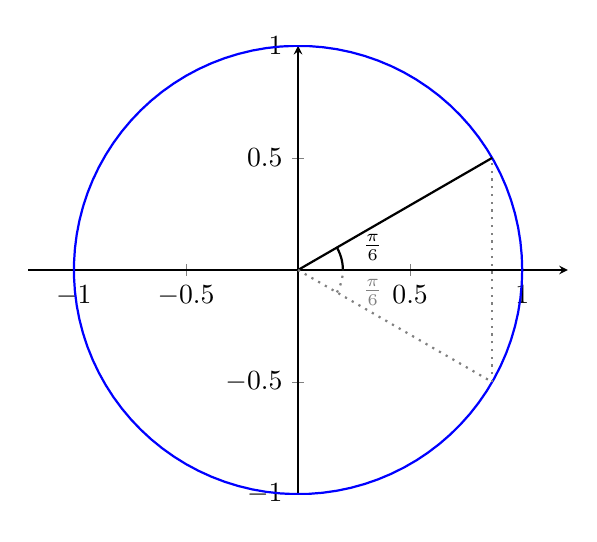
\begin{tikzpicture}
	\begin{axis}[xmin=-1,xmax=1,ymin=-1,ymax=1,axis x line=center,
	axis y line=center, axis equal]
	\addplot[blue,domain=0:2*pi,thick, samples=100] ({cos(deg(x))},{sin(deg(x))});
	\addplot[domain=0:sqrt(3)/2,thick] {1/sqrt(3)*x};
	\addplot[domain=0:pi/6,thick,samples=100] ({0.2*cos(deg(x))},{0.2*sin(deg(x))}) node[label={[label distance=2pt]0.5:\small$\frac{\pi}{6}$},pos=1] {};
	\addplot[domain=0:sqrt(3)/2,thick,gray,dotted] {-1/sqrt(3)*x};
	\addplot[domain=-pi/6:0,thick,samples=100,gray,dotted] ({0.2*cos(deg(x))},{0.2*sin(deg(x))}) node[label={[label distance=2pt]0.5:\small$\frac{\pi}{6}$},pos=0] {};
	\addplot[dotted,gray,thick] coordinates {(sqrt(3)/2, -1/2) (sqrt(3)/2, 1/2)};
	\end{axis}
	\end{tikzpicture}
	\caption{Opgave~\ref{it:trig3}}
	\label{fig:trig3}
\end{figure}

\item \label{it:trig4} I denne opgave beviser vi nogle af de eksakte værdier for sinus og cosinus til vinklen $ \frac{\pi}{4}$.
\begin{enumerate}
	\item Vis at $\sin(\frac{\pi}{4})=\frac{\sqrt{2}}{2}$ ved at regne på trekanten i Figur~\ref{fig:trig4}.(Hint: Pythagoras) 
	\item Brug idiotformlen til at vise at $\cos(\frac{\pi}{4})=\frac{\sqrt{2}}{2}$. 
\end{enumerate}

\begin{figure}
	\centering
	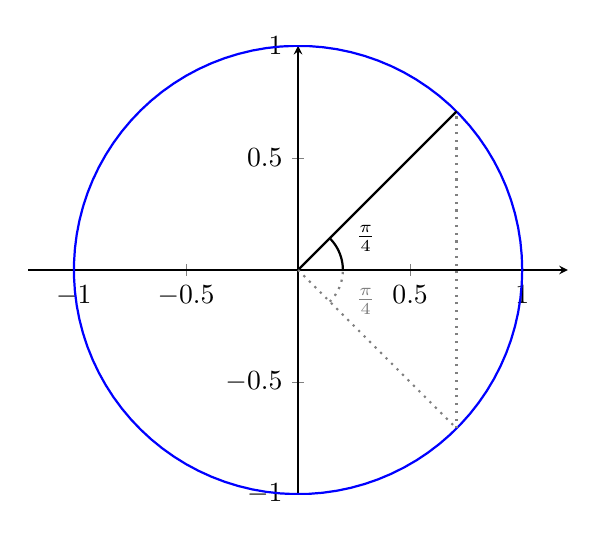
\begin{tikzpicture}
	\begin{axis}[xmin=-1,xmax=1,ymin=-1,ymax=1,axis x line=center,
	axis y line=center, axis equal]
	\addplot[blue,domain=0:2*pi,thick, samples=100] ({cos(deg(x))},{sin(deg(x))});
	\addplot[domain=0:sqrt(2)/2,thick] {1*x};
	\addplot[domain=0:pi/4,thick,samples=100] ({0.2*cos(deg(x))},{0.2*sin(deg(x))}) node[label={[label distance=2pt]0.5:\small$\frac{\pi}{4}$},pos=1] {};
	\addplot[domain=0:sqrt(2)/2,thick,gray,dotted] {-1*x};
	\addplot[domain=-pi/4:0,thick,samples=100,gray,dotted] ({0.2*cos(deg(x))},{0.2*sin(deg(x))}) node[label={[label distance=2pt]0.5:\small$\frac{\pi}{4}$},pos=0] {};
	\addplot[dotted,gray,thick] coordinates {({sqrt(2)/2}, -{sqrt(2)/2}) ({sqrt(2)/2}, {sqrt(2)/2})};
	\end{axis}
	\end{tikzpicture}
	\caption{Opgave~\ref{it:trig4}}
	\label{fig:trig4}
\end{figure}

\end{enumerate}
\section{Introduktion til differentialregning}
\begin{enumerate}
	\item Differentier funktionerne 
	\begin{align*}
	f_1(x)=2x+1,&& f_2(x)=x+\cos(x),&& f_3(x)=e^x-1,&&f_4(x)=\frac{1}{4}x^2+\ln(x).
	\end{align*}
	
	
	\item Bestem hældningen af funkionen $f(x)=x^3+x^2-x$ i punkterne $x=0$ og $x=1$.

	\item Brug regnereglen $\frac{d}{dx} x^n=nx^{n-1}$ til at differentiere funktionerne
	\begin{align*}
	f_1(x)=x^3,&& f_2(x)=\sqrt{x},&& f_3(x)=\frac{1}{x},&&f_4(x)=\frac{1}{x^2},&&f_5(x)=\frac{1}{\sqrt{x}}.
	\end{align*}
	\item \label{it:diff12} Bestem for hver af de blå grafer i Figur~\ref{fig:diff12} hvilken af de røde grafer der beskriver den afledede.
	
	\item Differentier funktionerne 
	\begin{align*}
	f(x)=3e^{2x}-\frac{1}{2}\ln x,&& g(x)=\frac{1}{2}\sin x,&& h(x)=\ln(\frac{x}{2})+3e^{-\frac{1}{6}x}.
	\end{align*}
	
	\item Differentier funktionerne
	\begin{align*}
	f(x)=x^7-2x^4-3x^2,&&g(x)=-x^5+4x^{\frac{3}{2}}-x^{-2},&&h(x)=\sqrt{x}+\frac{2}{x}.
	\end{align*}
	
	\begin{figure}
		\centering
		
		\begin{minipage}{0.3\linewidth}
			\begin{tikzpicture}[scale=0.5]
			\begin{axis}[xmin=-2,xmax=2,ymin=-2,ymax=2,axis x line=center,
			axis y line=center,ticks=none, restrict y to domain=-2:2]
			\addplot[thick,blue, samples = 600] {x^4-5/4*x^2+1/4};
			\end{axis}
			\end{tikzpicture}
		\end{minipage}
		\begin{minipage}{0.3\linewidth}
			\begin{tikzpicture}[scale=0.5]
			\begin{axis}[xmin=-2,xmax=2,ymin=-2,ymax=2,axis x line=center,
			axis y line=center,ticks=none]
			\addplot[thick,blue, samples = 200] {x+1/2};
			\end{axis}
			\end{tikzpicture}
		\end{minipage}
		\begin{minipage}{0.3\linewidth}
			\begin{tikzpicture}[scale=0.5]
			\begin{axis}[xmin=-2,xmax=2,ymin=-2,ymax=2,axis x line=center,
			axis y line=center,ticks=none, restrict y to domain=-2:2]
				\addplot[thick,blue, samples = 600] {x^3-x^2/2-x+1/2};
			\end{axis}
			\end{tikzpicture}
		\end{minipage}
%		
		\begin{minipage}{0.3\linewidth}
			\begin{tikzpicture}[scale=0.5]
			\begin{axis}[xmin=-2,xmax=2,ymin=-2,ymax=2,axis x line=center,
			axis y line=center,ticks=none]
				\addplot[thick,red, samples = 600] {3*x^2-x-1};
			\end{axis}
			\end{tikzpicture}
		\end{minipage}
		\begin{minipage}{0.3\linewidth}
			\begin{tikzpicture}[scale=0.5]
			\begin{axis}[xmin=-2,xmax=2,ymin=-2,ymax=2,axis x line=center,
			axis y line=center,ticks=none]
			\addplot[domain=-2:2,thick,red, samples = 600] {1};
			\end{axis}
			\end{tikzpicture}
		\end{minipage}
		\begin{minipage}{0.3\linewidth}
			\begin{tikzpicture}[scale=0.5]
			\begin{axis}[xmin=-2,xmax=2,ymin=-2,ymax=2,axis x line=center,
			axis y line=center,ticks=none, restrict y to domain=-2:2]
			\addplot[thick,red, samples = 200] {4*x^3-5/2*x};					
			\end{axis}
			\end{tikzpicture}
		\end{minipage}
		\caption{Opgave~\ref{it:diff12}}
		\label{fig:diff12}
	\end{figure}	
	
	
	\item Bestem, for hver af de følgende funktioner, de punkter hvor tangenthældningen er $2$.
	\begin{align*}
	f(x)=x^3+2x,&& f(x)=\frac{1}{3}x^3-3x^2+2x-1. 
	\end{align*}
	
	\item Differentier funktionerne 
	\begin{align*}
	f(x)=3\sqrt[3]{x},&& f(x)=(3x+4)x^2.
	\end{align*}
		

	\item Differentier funktionerne
	
	\begin{align*}
		f(x)=\frac{\sqrt{x}+1}{x},&& f(x)=\frac{x^2\sqrt{x^3}}{x^{-1/4}},&&f(x)=\ln\frac{1}{x^2}
	\end{align*}
	
	

	
	\item \label{it:diff11} Bestem for hver af de blå grafer i Figur~\ref{fig:diff11} hvilken af de røde grafer der beskriver den afledede.
		\begin{figure}
		\centering
		
		\begin{minipage}{0.3\linewidth}
			\begin{tikzpicture}[scale=0.5]
			\begin{axis}[xmin=-2,xmax=2,ymin=-2,ymax=2,axis x line=center,
				axis y line=center,ticks=none]
				\addplot[thick,blue, samples = 600] {e^(-x^2)};

				\end{axis}
			\end{tikzpicture}
		\end{minipage}
		\begin{minipage}{0.3\linewidth}
			\begin{tikzpicture}[scale=0.5]
			\begin{axis}[xmin=-2,xmax=2,ymin=-2,ymax=2,axis x line=center,
			axis y line=center,ticks=none,restrict y to domain=-2:2]
			\addplot[thick,blue, samples = 200] {1/(3*x)};
			\end{axis}
			\end{tikzpicture}
		\end{minipage}
			\begin{minipage}{0.3\linewidth}
		\begin{tikzpicture}[scale=0.5]
		\begin{axis}[xmin=-2,xmax=2,ymin=-2,ymax=2,axis x line=center,
		axis y line=center,ticks=none]
		\addplot[domain=-2:2,thick,blue, samples = 800] {x^4*cos(deg(x))};
		\end{axis}
		\end{tikzpicture}
	\end{minipage}

		\begin{minipage}{0.3\linewidth}
	\begin{tikzpicture}[scale=0.5]
	\begin{axis}[xmin=-2,xmax=2,ymin=-2,ymax=2,axis x line=center,
	axis y line=center,ticks=none,restrict y to domain=-2:2]
	\addplot[thick,red, samples = 200] {4*x^3*cos(deg(x))-x^4*sin(deg(x))};
	\end{axis}
	\end{tikzpicture}
\end{minipage}
\begin{minipage}{0.3\linewidth}
	\begin{tikzpicture}[scale=0.5]
	\begin{axis}[xmin=-2,xmax=2,ymin=-2,ymax=2,axis x line=center,
	axis y line=center,ticks=none,restrict y to domain=-2:2,restrict x to domain=-2:2]
	\addplot[,thick,red, samples = 200] {-2*x*e^(-x^2)};
	\end{axis}
	\end{tikzpicture}
\end{minipage}
\begin{minipage}{0.3\linewidth}
	\begin{tikzpicture}[scale=0.5]
	\begin{axis}[xmin=-2,xmax=2,ymin=-2,ymax=2,axis x line=center,
	axis y line=center,ticks=none,restrict y to domain=-2:2]
		\addplot[thick,red, samples = 600] {-1/(3*x^2)};
	\end{axis}
	\end{tikzpicture}
	\end{minipage}
	\caption{Opgave~\ref{it:diff11}}
	\label{fig:diff11}
	\end{figure}	
	

	
	\item Differentier funktionerne
	\begin{align*}
	f(x)=-\ln(\frac{1}{x^{-5}}),&& f(x)=\sqrt[3]{e^{9x}}.
	\end{align*}
	
	\end{enumerate}
\newpage
\section{Math101 exercises}
\begin{enumerate}

	\item Differentiate the functions:
	\begin{align*}
	f_1(x)=\sqrt{x^2+1},&& f_2(x)=\frac{x}{2x+1},&& f_3(x)=x\sin(x).
	\end{align*}

	\item Differentiate the functions:
	\begin{align*}
	f_1(x)=xe^x,&& f_2(x)=2x^2\cos(x),&& f_3(x)=\ln(x)e^x,&& f_4(x)=\sin(x)\cos(x).
	\end{align*}

	\item Differentiate the functions:
	\begin{align*}
	f_1(x)=\frac{x}{x-1},&&f_2(x)=\frac{x^2-x+1}{3x+2},&&f_3(x)=\frac{x^2}{x^3-2x^2}.
	\end{align*}
	
	\item Differentiate the functions:
	\begin{align*}
	f_1(x)=(3x-1)^\frac{4}{3},&& f_2(x)=\ln(x^2+3x),&& f_3(x)=e^{2-x},&&f_4(x)=\sin(x^3).
	\end{align*}
	
	\item \label{it:diff24}Determine the derivative of $f(x)=(x-1)e^x$.
	
	
	\item \label{it:diff23}Determine the derivative of $f(x)=x\ln(x)-x$.
	
	\item Differentiate the functions:
	\begin{align*}
	f_1(x)=e^{x^3},&&f_2(x)=\cos^2(x),&&f_3(x)=\sin^3(x)&&f_4(x)=2\tan(x^2).
	\end{align*}
		
	\item\label{it:diff21} Show that 
	\begin{align*}
	\frac{d}{dx} \tan x= 1+\tan^2x.
	\end{align*}
	(Hint: Use that $\tan x=\frac{\sin x}{\cos x}$)

	\item Differentiate the function $f(x)=\frac{xe^x}{\cos(x)}$.
		
	\item Differentiate the function
	\begin{align*}
	f(x)=\cos^2(\sqrt{x^2+1}).
	\end{align*}
		
	\item Differentiate the functions:
	\begin{align*}
	f_1(x)=\frac{\cos^2(x)}{\sin(x)},&&f_2(x)=\frac{e^{x^2}}{x},&&f_3(x)= \frac{x\cos(x)}{e^x}
	\end{align*}
	
	\item Differentiate the functions:
	\begin{align*}
	f(x)=\frac{x^2e^x}{-x\ln(x)},&& g(x)=xe^x\ln x,&& h(x)=\tan(x)e^{x}\cos(x)x^2
	\end{align*}
	
	
\end{enumerate}

\subsection{Opgaver}

\begin{enumerate}
	\item  Lad $A=\{1,2,3,4,5\}$ og $ B=\{ 3,5,\pi , 1,-1 \} $. Bestem en funktion $f\colon A\to B$ såedes at
	\begin{enumerate}
		\item $ f $ er injektiv og surjektiv.
%		\item $f $ er ikke injektiv men surjektiv.
%		\item $f$ er injektiv men ikke surjektiv.
		\item $f$ er hverken injektiv eller surjektiv.
	\end{enumerate}
	
	
	\item Kan cirklen med ligning $x^{2} +(y-1)^{2}=1$ beskrives som grafen af en funktion? Begrund dig svar, og i bekræftende tilfælde bedstem da funktionen.
	
	\item Givet mængderne 
	\begin{align*}
	A&= \{0,2,4,6,8\},\\
	B&=\{\text{Hund},\textup{Hest},\textup{Struds},\textup{Fugleedderkop},\textup{Laks},\textup{Mariehøne} \}
	\end{align*}
	bestem om følgende sammenhænge mellem $A$ og $B$ er funktioner. I bekræftende fald bestem også om de er injektive og/eller surjektive.
	\begin{enumerate}
		\item Lad $f\colon B\to A$ være givet ved
		\[f(x)=\textup{antal ben }x \textup{ har}.\]
		\item Lad $g$ være givet ved
		\begin{align*}
		g(0)&=\textup{Hund},\quad g(2)=\textup{Struds},\quad g(4)=\textup{Laks},\\ g(6)&=\textup{Fugleedderkop},\quad g(8)=\textup{Hest}
		\end{align*}
		
		\item Lad $ h\colon A\to B$ være givet ved at 
		\[h(x)= \textup{Dyerne i }B \textup{ som har } x \textup{ ben}.\] 
	\end{enumerate}

	\item Lad $f(x)=x^2-1$, $g(x)=\frac{1}{1+x}$. Bestem
	\begin{enumerate}
		\item $(f+g)(2)$
		\item $ \frac{f}{g}(-2) $
		\item $(fg)(0)$
		\item $\frac{g}{f}(x)$
		\item $(g-f)(x)$.
	\end{enumerate}

	\item Bestem værdimængden for funktionen $f\colon \mathbb{R}\to \mathbb{R}$ givet ved $f(x)=-3x^2+9$.
	
	\item \label{it:fun1} I Figur~\ref{fig:fun1} ses graferne for forskellige funktioner med definitionsmængde $[-2,2]$ og codomæne $[-2,2]$. Bestem for hver funktion om den er injektiv, surjektiv og/eller bijektiv.
	\begin{figure}
		\centering
	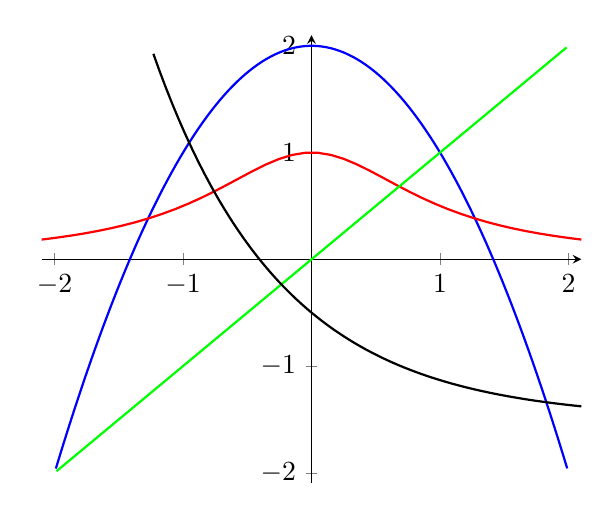
\begin{tikzpicture}
\begin{axis}[xmin=-2.1,xmax=2.1,ymin=-2.1,ymax=2.1,axis x line=center,
axis y line=center, restrict y to domain=-2:2]
\addplot[thick,blue,samples =300] {-x^2+2};
\addplot[thick,red,samples=100] {(1+x^2)^-1};
\addplot[thick,green, samples =200] {x };
\addplot[thick, black,samples=200] { e^-x -3/2};
\end{axis}
	\end{tikzpicture}
	\caption{Opgave~\ref{it:fun1}.}
	\label{fig:fun1}
	\end{figure}

	\item Bestem en mængde $D\subset \R$ således at funktionen $f\colon D\to \R$ givet ved $f(x)=x^2$ bliver injektiv.
	
	\item \label{it:fun2} På Figur~\ref{fig:fun2} ses grafen for funktionen $f(x)=x^{-1}$. Brug grafen til at afgøre om $f$ er injektiv, surjektiv og/eller bijektiv på $\R$. Hvis ikke $f$ er bijektiv bestem så det størst mulige domæne og codomæne således at $f$ bliver bijektiv.
	
	\begin{figure}
		\centering
		\begin{tikzpicture}
		\begin{axis}[xmin=-5,xmax=5,ymin=-20,ymax=20,axis x line=center,
		axis y line=center, restrict y to domain=-50:50]
		\addplot[thick,blue,samples=400] {1/x};
		\end{axis}
		\end{tikzpicture}
		\caption{Opgave~\ref{it:fun2}.}
		\label{fig:fun2}
	\end{figure}

	\item Brug \href{https://www.geogebra.org/m/eEE7RXzU}{Geogebra} til at bestemme for hvilke $a\in \{0,1,2,\dots,10\}$ funktionen $f\colon \R\to \R$ givet ved $f(x)=x^a$ er injektiv, surjektiv eller bijektiv. 
	
	\item Bestem den størst mulige definitionsmængde for funktionerne
	\begin{align*}
	f(x)=\sqrt{-x^2+x+2},&& g(x)=\frac{1}{(1+x^2)^\frac{1}{2}},&& h(x)=\frac{2}{\sqrt{x+2}}.
	\end{align*}
	
	\item \label{it:fun3exc} Figur~\ref{fig:fun3exc} viser forskellige kurver i planen. Argumenter for hvilke kurver der beskriver grafen for en funktion. 
	
 	\begin{figure}
		\centering
		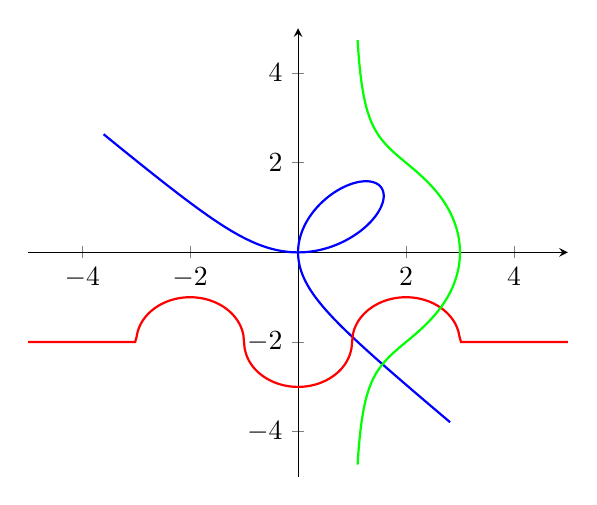
\begin{tikzpicture}[
		%declare function={func(\x)= (\x<-3)*(-2)+ and (\x>=-3,\x<=-1)*(sqrt(1-(x+2)^2)-2)+ and (\x>-1)*(-2); }
		declare function={
			func(\x)= (\x < -3) * (-2)   +
			and(x >= -3,\x<=-1) * (sqrt(1-(x+2)^2)-2)     +
			and(x >= -1,\x<=1) * (-sqrt(1-(x)^2)-2)     +
			and(x >= 1,\x<=3) * (sqrt(1-(x-2)^2)-2)     +
			(\x>3) * (-2)
			;
			}
		]
		\begin{axis}[xmin=-5,xmax=5,ymin=-5,ymax=5,axis x line=center,
	axis y line=center, restrict y to domain =-5:5]
		\addplot[data cs=polar, thick,blue,samples=200, domain= 0:180] ({x}, {3*sin(x)*cos(x)/(sin(x)^3+cos(x)^3)});
		\addplot[thick,red,samples=400] {func(x)};
		\addplot[data cs=polar, thick,green,samples=200, domain= 0:180] ({x}, {sec(x)+2*cos(x)});
		\end{axis}
		\end{tikzpicture}
		\caption{Opgave~\ref{it:fun3exc}.}
		\label{fig:fun3exc}
	\end{figure}

	\item Skitser grafen for en funktion som opfylder alle nedenstående puntker:
	\begin{enumerate}
		\item har domæne $[-2,4[$, og codomæne $[-2,4]$,
		\item går gennem punkterne $(-1,3)$ og $(2,-2)$,
		\item skærer y-aksen i $-2$,
		\item ikke skærer x-aksen.
		\end{enumerate}
	\item I \href{https://www.geogebra.org/m/eEE7RXzU}{Geogebra} er en kurve afbildet. Kurven afhænger af en parameter $a$. Bestem for hvilke (om nogen) $a\in \{-3,-2,\dots,2,3\}$ kurven beskriver grafen for en funktion.
\end{enumerate}

\subsection{Opgaver}

\begin{enumerate}
	
	\item Det oplyses at $f(1)=2$, $f(4)=1$, $g(1)=1$ og $g(2)=4$ for to funktioner $f$ og $g$. Bestem
	\begin{enumerate}
		\item $f(g(2))$
		\item $g(f(1))$
		\item $g(f(f(4)))$
	\end{enumerate}
	
	\item Lad $f,g$ være givet ved $f(x)=x^2$ og $g(x)=1/(1+x)$ på domænet $(0,\infty)$. Er $f\circ g=g\circ f$? 
	
	\item \label{it:ssfunk1} Lad $f(x)=x^2$ og $g(x)=\cos(x)$. På Figur~\ref{fig:ssfunk1} er graferne for $f\circ g$ of $g\circ f$ plottet. Bestem for hver graf den tilhørende funktionsforskrift.
	
	\begin{figure}
		\centering
		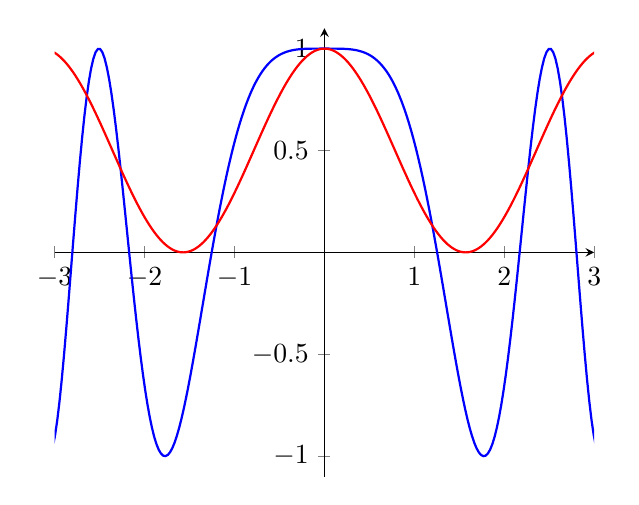
\begin{tikzpicture}
		\begin{axis}[xmin=-3,xmax=3,ymin=-1.1,ymax=1.1,axis x line=center,
		axis y line=center, restrict y to domain =-5:5]
		\addplot[thick,blue,samples=400] {cos(deg(x^2))};
		\addplot[thick,red,samples=400] {(cos(deg(x)))^2};
		\end{axis}
		\end{tikzpicture}
		\caption{Opgave~\ref{it:ssfunk1}}
		\label{fig:ssfunk1}
	\end{figure}
	
	\item Bestem $f\circ g$ og $g\circ f$ hvor $f(x)=\frac{1}{2}$ og $g(x)=4x^2+2x-1$.
	
	\item Lad $f\colon \{1,2,3\}\to \{a,b,c\}$ være givet ved $f(1)=b$, $ f(2)=a $, $ f(3)=c $. Bestem $g\colon \{a,b,c\}\to \{1,2,3\}$ så $g=f^{-1}$.
	
	\item Lad $f,g,h$ være funktioner defineret på $(0,\infty)$ givet ved
	\begin{align*}
	f(x)&=\sqrt{x},\\
	g(x)&=\frac{1}{1+x},\\
	h(x)&=\Big(\frac{1}{x}-1 \Big)^{2}.
	\end{align*}
	Bestem forskriften for følgende funktioner:
	\begin{enumerate}
		\item $f\circ g$,
		\item $g\circ f$,
		\item $f\circ h\circ g$,
		\item $g\circ h \circ f$,
		\item $ f\circ g \circ h $,
		\item $g\circ g$.
	\end{enumerate}
	
	
	\item Bestem den inverse funktion til $f\colon \R\setminus \{0\}\to \R\setminus\{0\}$ givet ved $f(x)=x^{-1}$. (Hint: Hvad er $f(f(x))$.)
	
	\item Vis at funktionerne $f\colon \R\setminus \{ \frac{1}{2}\}\to \R\setminus \{-\frac{1}{2} \}$ og $g\colon \R\setminus \{- \frac{1}{2}\} \to \R\setminus \{\frac{1}{2}\}$ givet ved
	\begin{align*}
	f(x)=\frac{x-1}{1-2x},&&g(x)=\frac{x+1}{1+2x},
	\end{align*}
	er inverse funktioner.
	
	\item Lad $f(x)=\cos((x-2)^2)$
	\begin{enumerate}
		\item Bestem funktioner $g$, $h$ så $f(x)=g(h(x))$.
		\item Bestem to andre funktioner $g_1$, $h_1$ så $f(x)=g_1(h_1(x))$
		\item Bestem tre funktioner $f_1,f_2,f_3$ så $f(x)=f_1(f_2(f_3(x)))$
	\end{enumerate}
	
	
	\item Lad funktionen $f(x)=e^{x^2}$ og bestem funktioner $g$ og $h$ så $f=g\circ h$.
	
	\item Lad $f\colon \R\to [-2,\infty[$ være givet ved $f(x)=(x-\sqrt{2})(x+\sqrt{2})$ og lad $g\colon [-2,\infty[\to [0,\infty[$ være givet ved $g(x)=\sqrt{x+2}$.
	\begin{enumerate}
		\item Bestem definitionsmængde, værdimængde og funktionsforskrift for $f\circ g$
		\item Er $g$ og $f$ inverse funktioner? (Hint: hvad er $(g\circ f)(-1)$?)
		\item Bestem en passende definitionsmængde $D$ så $f\colon D\to [-2,\infty[$ er invers til $g$.
	\end{enumerate}
	
		
	
	\item Betragt funktionerne $f\colon [0,\infty)\to [0,\infty)$ og $g\colon [0,\infty)\to[1,\infty)$ givet ved $f(x)=x^{3/2}$ og $g(x)=x^{2/3}+1$. 
	\begin{enumerate}
		\item Bestem det størst mulige domæne $D$ for funktionen $h\colon D\to \R$ givet ved $h(x)=x-1$ så sammensætningen $f \circ h$ er defineret.
		\item Vis at $g^{-1}=f\circ h$.
		\end{enumerate}
	
	%	
	
	
	
\end{enumerate}

\chapter{Repetition}\label{ch:rep}
Dette afsnit indeholder repetitionsopgaver som dækker de fleste af de emner der er gennemgået i disse noter. Hvis man kan løse disse opgaver uden de store problemer, så har man et fornuftigt udgangspunkt til at komme helskindet igennem diverse matematikkurser på Aalborg Universitet.
\section{Repetition}
\begin{enumerate}
	\item Svarene er:
	\begin{align*}
	-\frac{1}{12},&& \frac{1}{2},&& \frac{11}{6}.
	\end{align*}
	\item Svarene er:
	\begin{align*}
	x=25,&& x=2,x=-\frac{1}{2},&& x=1,x=-3,&& x=\pm 2,x=\pm \sqrt{2}.
	\end{align*}
	\item Svarene er:
	\begin{align*}
	\frac{x-2}{x+3},&& -\frac{x+3}{x+1}.
	\end{align*}
	\item Svarene er:
	\begin{align*}
	27x^6,&& y^-1,&& \sqrt{x}.
	\end{align*}
	\item Svarene er: 
\begin{align*}
x=2,y=\frac{-1}{2}.
\end{align*}
	\item $g$ er surjektiv men ikke injektiv og $f$ er hverken injektiv eller surjektiv.
	
	\item Svarene  $h(g(-1))=-1$ og $ g(f(3))=2 $.
	
	\item Svarene er
	\begin{align*}
	f(g(x))=\frac{1}{1+\cos^4(x)},&& g(f(x))=\cos^2(\frac{1}{1+x^2}).
	\end{align*}
	
	\item Svarene er:
	\begin{align*}
	6,&& 27,&& \frac{1}{\sqrt[3]{e}}.
	\end{align*}
	
	\item Svarene er:
	\begin{align*}
	x=1, && x=\frac{1}{2}.
	\end{align*}
	
	\item Svarene er:
	\begin{align*}
	\frac{3}{2},&& 3.
	\end{align*}
	
	\item Funkionen $f$ er kontinert på mængden $\R\setminus{0,1,2}$, altså i alle punkter undtagen 1,2 og 3.
	
	\item Svaret er: $\lim_{x\to 2} xe^{x^2-4}-x=0$.
	
	\item Svarene er:
	\begin{align*}
	f'(x)=4x+\frac{1}{2x^{\frac{3}{2}}},&&g'(x)=\frac{2}{3}x^{-\frac{1}{3}}+\sin(x),&& h'(x)=\frac{3}{2x}+4xe^{2x^2}.
	\end{align*}
	
	\item Svarene er:
	\begin{align*}
	f'(x)=2x(1+\tan^2(x^2)),&& g(x)=e^{2\sin(x)}(\sin(2x)+\cos(x)),&& h(x)=-\frac{1}{2}x^{-\frac{3}{2}}.
	\end{align*}
	
	
	\item\label{it:rep1ans} 	\begin{enumerate}
		\item Den første blå og den første røde hører sammen.
		\item Den anden blå og den tredje røde hører sammen.
		\item Den tredje blå og den anden røde hører sammen.
	\end{enumerate}
	
	\item Svaret er: $(f\circ g)'(3)=\frac{1}{4}-\frac{\pi}{6}$. 
	
	
 	\item\label{it:rep3} Det ses let at $f'(x)=2x-4$ så $f'(x)=0$ har løsningen $x=2$. Vælger vi punkterne $x_1=0$ og $x_2=3$ ser vi at $f'(x_1)=-4$ og at $f(x_2)=2$. Dette giver monotonilinjen som ses i Tabel~\ref{fig:mon1}. Vi ser dermed at $f$ er aftagende i intervallet $ ]-\infty,2] $ og voksende i intervallet $[2,\infty[$. Tangenten gennem punktet $(1,f(1))$ har forskriften
 	\begin{align*}
 	y=-2(x-1)+1=-2x+3.
 	\end{align*}
	
	\begin{table}[h!]
		\centering
		\begin{tabular}{@{}l  c c c@{}}
			$x$      & $0$ 		 & $2$				& $3$			\\ \toprule
			$f'(x)$  & $-4$		 &     $0$ 		 	& $2$			\\ \midrule
			$f(x)$   & $\searrow$&					& $\nearrow$	\\ \bottomrule  
		\end{tabular}
		\caption{Opgave~\ref{it:rep3}.}
		\label{fig:rep3}
	\end{table}
	
	
	
	\item Ved at undersøge kritiske punkter og interval endepunkter ses det at maksimumsværdien antages i $x=1$ samt at $f(1)=9$. Yderligere ses det at minimumsværdien tages i $x=-\frac{1}{3}$ samt at $f(-\frac{1}{3})=\frac{11}{3}$.
	
	\item\label{it:rep4} Lad $a$ og $b$ være givet som i Figur~\ref{fig:rep4} i.e.\ $b$ er højden af rektanglet og $a$ er halvdelen af længden. Ved at anvende trekantsberegninger får vi at
	\begin{align*}
	\tan(\frac{\pi}{3})=\frac{b}{\frac{1}{2}-a}.
	\end{align*}
	Isolerer vi $b$ får vi at
	\begin{align*}
	b=\frac{\sqrt{3}}{2}-\sqrt{3}a.
	\end{align*}
	Arealet af rektanglet kan dermed beskrives ved følgende funktion af $a$:
	\begin{align*}
	A(a)=2a(\frac{\sqrt{3}}{2}-\sqrt{3}a)=\sqrt{3}a-2\sqrt{3}a^2.
	\end{align*}
	Ved at anvende den sædvanlige optimeringsmetode finder vi at $A$ tager sit maksimum når $a=\frac{1}{4}$. Dette giver et maksimalt areal på $A(\frac{1}{4})=\frac{\sqrt{3}}{8}$. 
	
	
	
		\begin{figure}
			\centering
			\begin{tikzpicture}
			\begin{axis}[xmin=-0.2,xmax=1.1,ymin=-0.2,ymax=1.2,axis x line=center,
			axis y line=center, axis equal,xtick={0,1/2,1}]
			\addplot[blue,thick,domain=0:1/2] {sqrt(3)*x};
			\addplot[blue,thick,domain=1/2:1] {sqrt(3)-sqrt(3)*x};
			\addplot[blue,thick,domain=0:1] {0};
			
			\addplot[thick,red,domain=1/4:3/4] {0} node [pos=0.25,label=above: $a$] {}  node [pos=0.75,label=above: $a$] {} ;
			\addplot[thick,red,domain=1/4:3/4] {sqrt(3)/4};
			\addplot[thick,red] coordinates {({0.25},0) ({0.25},{sqrt(3)*0.25}) } node [pos=0.5,label=left: $b$] {};
			\addplot[thick,red] coordinates {({0.75},0) ({0.75},{sqrt(3)*0.25}) } node [pos=0.5,label=right: $b$] {};
			\end{axis}
			\end{tikzpicture}
			\caption{Opgave~\ref{it:rep4}}
			\label{fig:rep4}
		\end{figure}
	
	
	
	
	\item Nej.
	

	\item Svarene er:
	\begin{align*}
	\frac{1}{3}x^3+x+c,&& \frac{2}{3}x^{\frac{3}{2}}-\cos(x)+c,&& e^{\frac{x}{2}}+c.
	\end{align*}

	\item Svarene er:
	\begin{align*}
	x\sin(x)+\cos(x)+c,&& \frac{1}{3}x^3\ln(x)-\frac{1}{9}x^3+c.
	\end{align*}
	
	\item Svarene er:
	\begin{align*}
	e^{x^3+3x-1}+c,&& \frac{1}{2}(x^2\ln(x^2)-x^2)+c, && -e^{-(x^4+x^2-x)}+c.
	\end{align*}
	
	\item Svarene er:
	\begin{align*}
	\frac{8}{3},&& 0,&& 2e^{-1}-1.
	\end{align*}
	
	\item Udregn følgende bestemte integraler:
	\begin{align*}
	1-e,&& 0.
	\end{align*}
	
	\item\label{it:rep2ans} Vi har at
	\begin{align*}
	\int_0^{2\pi} f(x)\dd x&=\int_0^{\frac{\pi}{4}} \cos(x)-\sin(x) \dd x+\int_{\frac{\pi}{4}}^{\frac{5\pi}{4}} \sin(x)-\cos(x)\dd x+\int_{\frac{5\pi}{4}}^{2\pi} \cos(x)-\sin(x)\dd x\\
	&=[\sin(x)+\cos(x)]_{0}^{\frac{\pi}{4}}+[-\cos(x)-\sin(x)]_{\frac{\pi}{4}}^{\frac{5\pi}{4}}+[\sin(x)+\cos(x)]_{\frac{5\pi}{4}}^{2\pi}\\
	&=(\sqrt{2}-1)+(\sqrt{2}+\sqrt{2})+(1+\sqrt{2})\\
	&=4\sqrt{2}.
	\end{align*}
	
	\item Den fuldstændige løsning er $y(x)=ce^{-3x}$ hvor $c\in \R$. Da man blot bliver bedt om at finde en løsning kunne man være doven og vælge $y(x)=0$.
	
	\item Ved at anvende kædereglen ses at $ f'(x)=-e^x e^{-e^x} $. Indsætter vi $f$ og $f'$ i differentialligningen får vi
	\begin{align*}
	-\frac{f'(x)}{f(x)}=-\frac{-e^xe^{-e^x}}{e^{-e^x}}=-(-e^x)=e^x.
	\end{align*}
	
	\item Funktionerne $y_1$ og $y_2$ er løsninger.
	
	\item Tangentligningen har forskriften $y=\ln(2)$.
	
	\item Vi har at
	\begin{align*}
	y_1'(x)&=\frac{d}{dx}\cos(x)=-sin(x)=-y_2(x)\\
	y_2'(x)&=\frac{d}{dx}\sin(x)=\cos(x)=y_1(x).
	\end{align*}
	Derudover er det velkendt at  $\cos(0)=1$ og $\sin(0)=0$. 
	
	\item Bruger vi Panzerformlen får vi at
	\begin{align*}
	y(x)=e^{-\frac{1}{2}x^2}\int xe^{\frac{1}{2}x^2}\dd x +ce^{-\frac{1}{2}x^2}=e^{-\frac{1}{2}x^2}e^{\frac{1}{2}x^2}+ce^{-\frac{1}{2}x^2}=1+ce^{-\frac{1}{2}x^2}.
	\end{align*}

	
	\item Bruger vi Panzerformlen får vi at
	\begin{align*}
	y(x)=e^{-\cos(x)}\int \sin(x)e^{\cos(x)}\dd x+ce^{-\cos(x)}=e^{-\cos(x)}(-e^{\cos(x)})+ce^{-\cos(x)}=ce^{-\cos(x)}-1.
	\end{align*}
	
	\item Funktionerne $y_1$, $y_3$ og $y_4$ løser differentialligningen.
	
	\item Svarene er:
	\begin{align*}
	\begin{bmatrix}
	-4\\2
	\end{bmatrix},&&\begin{bmatrix}
	-2\\-4
	\end{bmatrix},&&\begin{bmatrix}
	3\\-4
	\end{bmatrix},&&\begin{bmatrix}
	7\\4
	\end{bmatrix},&&2\sqrt{5},&&\sqrt{5},&&0,&& 0.
	\end{align*}
	
	\item Arealet er $5$.
	
		
	\item Vi har at
	\begin{align*}
	\vec{u}\cdot \vec{v}=-\Big(\frac{\sqrt{2}}{2}\Big)^2+\Big(\frac{\sqrt{2}}{2}\Big)^2=0,
	\end{align*}
	samt at
	\begin{align*}
	\norm{\vec{u}}&=\sqrt{\Big(\frac{\sqrt{2}}{2}\Big)^2+\Big(-\frac{\sqrt{2}}{2}\Big)^2}=\sqrt{\frac{1}{2}+\frac{1}{2}}=1,\\
	\norm{\vec{v}}&=\sqrt{\Big(-\frac{\sqrt{2}}{2}\Big)^2+\Big(-\frac{\sqrt{2}}{2}\Big)^2}=\sqrt{\frac{1}{2}+\frac{1}{2}}=1,
	\end{align*}
	
	\item Nej.
	
	\item  	\item Svarene er:
	\begin{align*}
	\begin{bmatrix}
	-1\\1\\-2
	\end{bmatrix},&&\begin{bmatrix}
	0\\-2\\6
	\end{bmatrix},&&\begin{bmatrix}
	1\\0\\-1
	\end{bmatrix},&&\begin{bmatrix}
	1\\-2\\5
	\end{bmatrix},&&\sqrt{6},&&\sqrt{10},&&-7,&& \begin{bmatrix}
	1\\3\\1
	\end{bmatrix}.
	\end{align*}
	
	\item Arealet er $ 6\sqrt{3}$.
	
	\item Bestem en parameterfremstilling for linjen $m$ gennem punkterne $P_1 =
	(2, 3,-1)$ og $P_2 = (2,-2, 0)$. Ligger $P = (2, 8, -2)$ på $m$?
	
	\item En mulig parameterfremstilling er
	\begin{align*}
	\begin{bmatrix}
	x\\y\\z
	\end{bmatrix}=\begin{bmatrix}
	2\\-2\\0
	\end{bmatrix}+t \begin{bmatrix}
	0\\5\\-1
	\end{bmatrix}.
	\end{align*}
	$P$ ligger på linjen.
	
	
	En mulig ligning for planen er
	\begin{align*}
	2x-y+3z-4=0
	\end{align*}
	Punktet $P_1$ ligger i planen.
	
\end{enumerate}

\chapter{Facit}
\section{Brøker}

\begin{enumerate}
\item Svarene er:
\begin{align*}
\frac{8}{4},&& \iffalse \frac{20}{4},&&  \frac{2}{4},&& \fi \frac{10}{4},&& \frac{4 \pi}{4},&& \frac{6}{4}.% ,&& \frac{3}{4},&&\frac{120}{4}.
\end{align*}
\item Svarene er:
\begin{align*}
\frac{21}{3},&& \iffalse \frac{9}{3},&&\frac{1}{3},&& \fi \frac{2}{3},&&\frac{4}{3},&&\frac{12\pi}{3 }.% && \frac{2}{3},&&\frac{3}{3e}.
\end{align*}
\item Svarene er:
\begin{align*}
2,&& \frac{5}{4},&& \frac{13}{12},&&1,&&-\frac{1}{3}.
\end{align*}
\item Svarene er:
\begin{align*}
\frac{3}{2},&&\frac{1}{12},&& \frac{7}{24},&& \frac{3}{10},&& \frac{14}{9},&&\frac{9}{25}.
\end{align*}
\item Svarene er:
\begin{align*}
4,&& \frac{3}{2},&& \frac{1}{4},&& 1,&& \frac{5}{4}.
\end{align*}
\item Svarene er:
\begin{align*}
x+1,&& x+2y,&& 2x+7,&&y,&& \frac{x+3}{2x},&& \frac{x-1}{3x}.
\end{align*}
\item Svarene er:
\begin{align*}
\frac{73}{50},&& -11,&& \frac{5}{8},&& 0,&& \frac{19}{2}.
\end{align*}
\item Svaret er:
\begin{align*}
1.
\end{align*}
\item Svarene er:
\begin{align*}
\frac{1}{2}= \frac{3}{6},&& \frac{6}{7}=\frac{42}{49},&& \frac{2x}{y}=\frac{2xy}{y^2},&& \frac{ \pi}{\sqrt{2}}=\frac{3\pi^3}{3 \pi^2 \sqrt{2}}.
\end{align*}
\item Svarene er:
\begin{align*}
\frac{9}{11},&& 14,&&\frac{1}{11}.
\end{align*}
\item Svaret er:
\begin{align*}
6.
\end{align*}
\item Vi regner på venstresiden og får
\begin{align*}
\frac{ \frac{1}{b}+1 }{1- \frac{a}{b}}=\frac{b}{b}\frac{ \frac{1}{b}+1 }{1- \frac{a}{b}}=\frac{1+b}{b-a},
\end{align*}
hvor $b\notin \{0,a\}$.
\item Vi regner på venstresiden og får
\begin{align*}
\frac{ \frac{a}{b}+1}{ \frac{b}{a}+1}=\frac{ \frac{a}{b}+\frac{b}{b} }{ \frac{b}{a}+\frac{a}{a} }=\frac{a+b}{b}\c \frac{a}{a+b}=\frac{a}{b}.
\end{align*}
hvor $a,b\neq 0$
\end{enumerate}

\section{Kvadratsætninger}
\begin{enumerate}
\item Svarene er:
\begin{align*}
x^2+1+2x,&& 4x^2+9-12x,&& x^2,&& 9a^2+4b^2-6ab.
\end{align*}
\item Svarene er:
\begin{align*}
\frac{x+3}{2x},&& \frac{2x+3}{2x-3},&& \frac{2x+6}{x},&& \frac{x-2y}{2}.
\end{align*}
\item Centrumskoordinaterne og radierne er:
\begin{align*}
(0,0), r=1,&& (1,-1), r=5,&& (-2,0), r=2.
\end{align*}
\item Vi har at
\begin{align*}
99^2-101^2&=(99-101)(99+101)=-2(200)=-400,\\
999^2&=(1000-1)^2=1000^2+1^2-2000= 998001,\\
499^2-501^2&=(499-501)(499+501)=-2(1000)= -2000,\\ 
99998^2-100002^2&=(99998-100002)(99998+100002)=-4(200000)=-800000.
\end{align*}
\item Ved at reducere fås
\begin{align*}
8-4a,&& 2x,&&2x-3.
\end{align*}
\item Centrumskoordinaterne og radierne er:
\begin{align*}
(3,4),r=5,&& \Big( \frac{1}{2},-\frac{1}{2}\Big), r=1.
\end{align*}
\item \label{it:1ans} Arealet af figuren i Figur~\ref{fig:1} er $(a+b)^2$ hvilket figuren viser kan beskrives som $a^2+b^2+2ab$.
\item \label{it:2ans} Den højre del af Figur~\ref{fig:2} viser, at summen af det grå areal og det skraverede areal er $(a+b)(a-b)$. Den venstre figur viser, at dette areal er det samme som $a^2-b^2$.
\item \label{it:3ans} Det totale areal som ses i Figur~\ref{fig:3} kan beskrives både som $(a+b)^2$ og som $c^2+4( 1/2) ab$. Dette giver ligningen
\begin{align*}
c^2+4 \frac{1}{2}ab=(a+b)^2,
\end{align*}
som kan reduceres til $c^2=a^2+b^2$.

\item Svarene er:
\begin{align*}
a^2+36b^2+12ab,&& 16-a^2,&& x^2+\frac{1}{x^2}+2.
\end{align*}
\item Ved at sætte brøkerne på fælles nævner fås
\begin{align*}
\frac{7a +b}{4a^2-4b^2}-\frac{3}{4a+4b}-\frac{3}{4a-4b}&=\frac{7a+b-3(a-b)-3(a+b)}{4(a-b)(a+b)}\\
&=\frac{a+b}{4(a-b)(a+b)}\\
&=\frac{1}{4a-4b}.
\end{align*}
\item \label{it:4ans} Lader vi $d=b+c$ får vi
\begin{align*}
(a+b+c)^2= a^2+d^2+2ad&= a^2+(b+c)^2+2a(b+c)\\&=a^2+b^2+c^2+2bc+2ab+2ac.
\end{align*}
\item \label{it:ex13ans} Dividerer vi med $a$ får vi
\begin{align*}
x^2+\frac{b}{a}x+\frac{c}{a}=0.
\end{align*}
Hvis vi skal omskrive dette så vi får en parentes $(x+k)^2$ på venstresiden må $\frac{b}{a}x$ være det dobbelte produkt hvilket betyder, at
\begin{align*}
k=\frac{b}{2a}.
\end{align*}
For at samle parentesen skal vi så lægge $k^2$ til på begge sider, hvilket giver
\begin{align*}
x^2+2\frac{b}{2a} x+\frac{b^2}{4a^2}+\frac{c}{a}=\frac{b^2}{4a^2}.
\end{align*}
Samler vi parentesen og reducerer får vi
\begin{align*}
\Big( x+\frac{b}{2a}\Big)^2=\frac{b^2-4ac}{4a^2},
\end{align*}
hvilket medfører at $d=b^2-4ac$.

% \begin{figure}
% \centering
% \begin{tikzpicture}
% \draw (0,0)--(5,0)--(5,5)--(0,5)-- cycle;
% \draw[dashed] (0,4)--(5,4);
% \draw[dashed] (4,0)--(4,5);
% \node at (2,0) [label=below: $a$] {};
% \node at (4.5,0) [label=below:$b$] {};
% \node at (0,2) [label=left: $a$] {};
% \node at (0,4.5) [label=left:$b$] {};
% \node at (2,5) [label=above: $a$] {};
% \node at (4.5,5) [label=above:$b$] {};
% \node at (5,2) [label=right: $a$] {};
% \node at (5,4.5) [label=right:$b$] {};
% \end{tikzpicture}
% \caption{Opgave~\ref{it:1}}
% \label{fig:1ans}
% \end{figure}
% %
% \begin{figure}
% \centering
% \begin{tikzpicture}
% \draw (0,0)--(0,4)--(4,4)--(4,0)--cycle;
% \draw[pattern=north east lines] (0,0)--(3,0)--(3,1)--(0,4)--cycle;
% \draw[fill=gray] (3,1)--(0,4)--(4,4)--(4,1)--cycle;
% \node at (1.5,0) [label=below: $a-b$] {};
% \node at (3.5,0) [label=below:$b$] {};
% \node at (0,2) [label=left: $a$] {};
% \node at (2,4) [label=above: $a$] {};
% \node at (4,2.5) [label=right: $a-b$] {};
% \node at (4,0.5) [label=right:$b$] {};
% %%%Newfig
% \draw (8,0)--(11,0)--(11,5)--(8,5)--cycle;
% \draw[pattern=north east lines] (8,0)--(8,4)--(11,1)--(11,0)--cycle;
% \draw[fill=gray] (8,4)--(8,5)--(11,5)--(11,1)-- cycle;
% \node at (9.5,0) [label=below: $a-b$] {};
% \node at (8,2) [label= left: $a$] {};
% \node at (8,4.5) [label= left: $b$] {};
% \node at (9.5,5) [label= above: $a-b$] {};
% \node at (11,3) [label= right: $a$] {};
% \node at (11,0.5) [label= right: $b$] {};
% \end{tikzpicture}
% \caption{Opgave~\ref{it:2}}
% \label{fig:2ans}
% \end{figure}
% \begin{figure}
% \centering
% \begin{tikzpicture}[auto]
% \draw (0,0)--(0,5)--(5,5)--(5,0)--cycle;
% \draw (0,3)-- node {$c$} (2,0) ;
% \draw (0,3)--node {$c$} (3,5);
% \draw (3,5)--node {$c$} (5,2);
% \draw (2,0)-- node {$c$} (5,2);
% \node at (1,0) [label=below: $a$] {};
% \node at (3.5,0) [label=below: $b$] {};
% \node at (0,1.5) [label=left: $b$] {};
% \node at (0, 4) [label=left: $a$] {};
% \node at (1.5,5) [label=above: $b$] {};
% \node at (4,5) [label=above: $a$] {};
% \node at (5,1)  [label= right: $a$] {};
% \node at (5,3.5) [label=right: $b$] {};
% \end{tikzpicture}
% \caption{Opgave~\ref{it:3}}
% \label{fig:3ans}
% \end{figure}
\end{enumerate}
\newpage
\section{Math101 facit til 3. gang}
\begin{enumerate}
	
	\item Svarene er: $f(-1)=2$ og $f(2)=17$.
	
	\item Svarene er:
	\begin{itemize}
		\item Nej fordi i såfald skulle $f(0)$ være lig med både $2$ og $0$ samtidig.
		\item $f_+(x) = 1+\sqrt{1-x^2}$.
		\item $f_-(x) = 1-\sqrt{1-x^2}$
	\end{itemize}	
	
	\item Svaret er $(f\circ g)(x)=x$.
	

	\item Svarene er:
	\begin{align*}
	D(f)=\R\setminus\{1\},&& D(g)=\R\setminus \{-1,1\},&& D(h)=[\frac{3}{2},\infty[.
	\end{align*}	
	
	\item  Svarene er $(f\circ g)(1)=\frac{\sqrt{2}}{2}$ og $(g\circ f)(1)=\frac{1}{2}$, hvorfor $f\circ g\neq g\circ f$?
	
	\item Skæringspunktet er $(\frac{1}{4},\frac{7}{4})$.	
	
		\item Svarene er $(f\circ g)(x)=1$ og $(g\circ f)(x)=5$.
	
		\item Svarene er:
	\begin{align*}
	D(f)=\R,&& D(g)=\R\setminus\{1,3\},&& D(h)=[0,2].
	\end{align*}
	
	
	

	\item Tag $f(x)=e^x$ og $g(x)=2x^2-1$.
	
	\item Skæringspunktet er $(-1,1)$.
	
	\item Tag $f(x)=x^2$, $g(x)=\sin(x)$ og $h(x)=3x$.
	
	\item Svarene er:
	\begin{align*}
	f(g(x))=\frac{3x^2}{(1-2x)^2},&& f(h(x))=\frac{3}{x},&& h(g(x))=\frac{1}{\sqrt{x}}+2,\\ h(f(x))=\sqrt{3}\frac{1}{x-2}+2,&&g(f(h(x)))=\frac{x}{3}.
	\end{align*} 
	
		\item Nej.
	
	\item \label{it:fun5} I Figur~\ref{fig:fun5} ses en funktion som opfylder:
	\begin{enumerate}
		\item har domæne $[-1,1]$,
		\item går gennem punkterne $(-1,0)$ og $(1,1)$,
		\item skærer $y$-aksen i $-1$,
	\end{enumerate}
	Bemærk at der findes mange korrekte svar.
	
	\begin{figure}
		\centering
		\begin{tikzpicture}
		\begin{axis}[xmin=-1,xmax=1,ymin=-1,ymax=1,axis x line=center,
		axis y line=center, restrict y to domain =-5:5]
		\addplot[thick,blue,samples=200, domain= -1:0] {-x-1};
		\addplot[thick,blue,samples=200, domain= 0:1] {(2*x-1)};
		\end{axis}
		\end{tikzpicture}
		\caption{Opgave~\ref{it:fun5}.}
		\label{fig:fun5}
	\end{figure}
\end{enumerate}
\newpage
\section{Math101 answers}
\begin{enumerate}
	\item The answers are:
	\begin{align*}
	27,&& \frac{1}{2}, &&-1,&&8,&&1.
	\end{align*}
	\item The answers are:
	\begin{align*}
	7,&& 2,&& -2,&& 3,&&0.
	\end{align*}
	
	\item The answers are:
	\begin{align*}
	\sqrt{2},&& \frac{3\sqrt{3}}{2},&& \frac{2}{\sqrt{3}}.
	\end{align*}
	

	\item The answers are:
	\begin{align*}
	3,&&1,&& 3
	\end{align*}
	
	\item The answers are:
	\begin{align*}
	-\frac{\sqrt{2}}{2},&& -\frac{\sqrt{3}}{2},&&-1,&& -\frac{1}{2}.
	\end{align*}
	
	
	\item The answers are:
	\begin{align*}
	\frac{3}{2}\ln(2),&& 2,&& \frac{1}{2}.
	\end{align*}
	
	
	\item The answers are:
	\begin{align*}
	1,&&3e,&& \frac{1}{7},&& \frac{7}{9},&& \frac{1}{9}.
	\end{align*}
	
	\item The answers are:
	\begin{align*}
	\frac{1}{2},&& 0,&& -1,&& 0.
	\end{align*}
	
	
	\item The answers are: 
	\begin{align*}
	x=\ln(3),&& x=e^4,&& x=18,&& x=3.
	\end{align*}
	

	\item he answers could be:
	\begin{align*}
	x=\frac{\pi}{4},x=\frac{3\pi}{4},&& x=\frac{\pi}{6},x=-\frac{\pi}{6},&& x=\frac{2\pi}{3},x=\frac{4\pi}{3}.
	\end{align*}
	Note that there are infinitely many correct answers.

	\item \label{it:trig3} The answers could be:

\begin{enumerate}
	\item The triangle in Figure~\ref{fig:trig3} is equilateral since all angles are $\frac{\pi}{3}$. Since two sides of the triangle has length $1$ it follows that the last side must be of length $1$. Hence it follows that $\sin(\frac{\pi}{6})$, which is half of the dotted line, must be $\frac{1}{2}$.
	
	\item The Pythagorean trigonometric identity gives that $\sin^2 \frac{\pi}{6}+\cos^2\frac{\pi}{6}=1$ and solving for $\cos(\frac{\pi}{6})$ gives that $ \cos(\frac{\pi}{6})=\sqrt{1-\frac{1}{4}}=\frac{\sqrt{3}}{2} $.
	
	\item Using the hint we obtain that
	\begin{align*}
	\sin(\frac{\pi}{3})=\sin(2\frac{\pi}{6}) =2\sin(\frac{\pi}{6})\cos(\frac{\pi}{6})=2\frac{1}{2}\frac{\sqrt{3}}{2}=\frac{\sqrt{3}}{2}.
	\end{align*}
	
	\item It follows that
	\begin{align*}
	\sin^2 \frac{\pi}{3}+ \cos^2\frac{\pi}{3}=1\quad \Leftrightarrow\quad \cos^2\frac{\pi}{3}=1-\frac{3}{4}\quad \Leftrightarrow\quad \cos\frac{\pi}{3}=\sqrt{\frac{1}{4}}=\frac{1}{2}.
	\end{align*}
	
\end{enumerate}

\begin{figure}
	\centering
	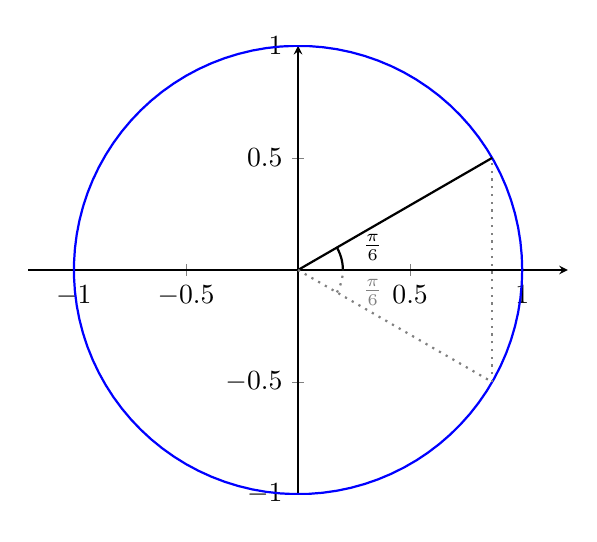
\begin{tikzpicture}
	\begin{axis}[xmin=-1,xmax=1,ymin=-1,ymax=1,axis x line=center,
	axis y line=center, axis equal]
	\addplot[blue,domain=0:2*pi,thick, samples=100] ({cos(deg(x))},{sin(deg(x))});
	\addplot[domain=0:sqrt(3)/2,thick] {1/sqrt(3)*x};
	\addplot[domain=0:pi/6,thick,samples=100] ({0.2*cos(deg(x))},{0.2*sin(deg(x))}) node[label={[label distance=2pt]0.5:\small$\frac{\pi}{6}$},pos=1] {};
	\addplot[domain=0:sqrt(3)/2,thick,gray,dotted] {-1/sqrt(3)*x};
	\addplot[domain=-pi/6:0,thick,samples=100,gray,dotted] ({0.2*cos(deg(x))},{0.2*sin(deg(x))}) node[label={[label distance=2pt]0.5:\small$\frac{\pi}{6}$},pos=0] {};
	\addplot[dotted,gray,thick] coordinates {(sqrt(3)/2, -1/2) (sqrt(3)/2, 1/2)};
	\end{axis}
	\end{tikzpicture}
	\caption{Exercise~\ref{it:trig3}}
	\label{fig:trig3}
\end{figure}

\item \label{it:trig4} The answers could be:
\begin{enumerate}
	\item The triangle in Figure~\ref{fig:trig4} is a right triangle where each leg has length $1$. Using the Pythagorean theorem it follows that the hypotenuse must have length $\sqrt{1+1}=\sqrt{2}$. singe $\sin \frac{\pi}{4}$ is half the length of the hypotenuse we have that $\sin\frac{\pi}{4}=\frac{\sqrt{2}}{2}$. 
	\item It follows that
	\begin{align*}
	\cos \frac{\pi}{4}=\sqrt{1-\frac{1}{2}}=\frac{\sqrt{2}}{2}.
	\end{align*}
\end{enumerate}

\begin{figure}
	\centering
	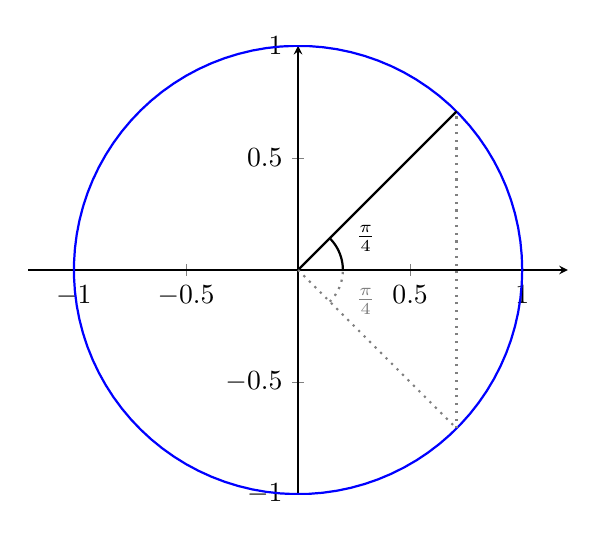
\begin{tikzpicture}
	\begin{axis}[xmin=-1,xmax=1,ymin=-1,ymax=1,axis x line=center,
	axis y line=center, axis equal]
	\addplot[blue,domain=0:2*pi,thick, samples=100] ({cos(deg(x))},{sin(deg(x))});
	\addplot[domain=0:sqrt(2)/2,thick] {1*x};
	\addplot[domain=0:pi/4,thick,samples=100] ({0.2*cos(deg(x))},{0.2*sin(deg(x))}) node[label={[label distance=2pt]0.5:\small$\frac{\pi}{4}$},pos=1] {};
	\addplot[domain=0:sqrt(2)/2,thick,gray,dotted] {-1*x};
	\addplot[domain=-pi/4:0,thick,samples=100,gray,dotted] ({0.2*cos(deg(x))},{0.2*sin(deg(x))}) node[label={[label distance=2pt]0.5:\small$\frac{\pi}{4}$},pos=0] {};
	\addplot[dotted,gray,thick] coordinates {({sqrt(2)/2}, -{sqrt(2)/2}) ({sqrt(2)/2}, {sqrt(2)/2})};
	\end{axis}
	\end{tikzpicture}
	\caption{Exercise~\ref{it:trig4}}
	\label{fig:trig4}
\end{figure}

\end{enumerate}
\section{Ligninger og uligheder}
\begin{enumerate}
\item Svarene er:
\begin{align*}
x=3,&& x=-3,&&x=6,&& x=\frac{-3}{4}.
\end{align*}

\item Svarene er:
\begin{align*}
x=-1,&& x=12,&& x=\frac{-7}{2}.
\end{align*}

\item Svarene er: 
\begin{align*}
x<\frac{4}{7},&& x>\frac{5}{2},&& \textup{ingen løsning},&& \frac{7}{2}\leq x.
\end{align*}

\item Svarene er:
\begin{enumerate}
\item $a\neq -1, b\in \mathbb{R}$
\item $a=-1,b\neq 4$
\item $a=-1,b=4$.
\end{enumerate}

\item Svarene er:
\begin{align*}
 \textup{ingen løsning},&& x\in \mathbb{R}.
\end{align*}

\item Svarene er:
\begin{align*}
x=\frac{11}{5},&& x=1,&& x=\frac{7}{2},&& x=-3.
\end{align*}

\item Svarene er:
\begin{align*}
x=\frac{13}{4},&& x=\frac{6}{11}.
\end{align*}

\item Svarene er:
\begin{align*}
x=2\sqrt{2},&& x=\frac{\pi+3}{\pi-\sqrt{2}},&&x=\frac{5}{2}.
\end{align*}

\item Svarene er:
\begin{enumerate}
	\item Kvadrat med hjørner $(0,0),(2,0),(0,2),(2,2)$.
	\item Cirkelskive med centrum $(0,0)$ og $r=2$.
	\item Trapez med hjørner $(0,0),(0,2),(2,6),(2,0)$.
\end{enumerate}


\item Svarene er:
\begin{enumerate}
	\item Rektangel: $ -4\leq x\leq -2 $, $ 0\leq y\leq 4 $.
	\item Cirkelskive: $ (x+2)^2+(y+3)^2\leq 4 $.
	\item Trekant: $ 0\leq x\leq 4 $, $ \frac{1}{2}x\leq y\leq 2 $, eller $0\leq y\leq 2$, $ 0\leq x\leq 2y $.
\end{enumerate}
%\begin{figure}
%\centering
%\begin{tikzpicture}
%\draw[help lines, color=gray!30, dashed] (-4.9,-4.9) grid (4.9,4.9);
%\draw[->,ultra thick] (-5,0)--(5,0) node[right]{$x$};
%\draw[->,ultra thick] (0,-5)--(0,5) node[above]{$y$};
%
%\draw[fill=gray] (-2,-3) circle (2);
%\draw[fill=gray] (0,0)--(0,2)--(4,2)--cycle;
%\draw[fill=gray] (-4,0)--(-2,0)--(-2,4)--(-4,4)--cycle;
%\end{tikzpicture}
%\caption{Find uligheder der beskriver de grå områder.}
%\label{fig:ligninger1}
%\end{figure}

\item Det er klart at $0\leq (a-b)^2$. Bruger vi kvadratsætningerne har vi
\begin{align*}
0 \leq (a-b)^2=a^2+b^2-2ab.
\end{align*}
Ved at flytte lidt rundt på ovenstående ulighed får vi
\begin{align*}
ab\leq \frac{a^2}{2}+\frac{b^2}{2}.
\end{align*}
Bemærk der findes uendeligt mange valg af $a,b,c,d$. Et muligt kunne være $a=1$, $b=1$, $c=0$, $d=1$.


\item Bruger vi kvadratsætningerne får vi
\begin{align*}
(\sqrt{a}+\sqrt{b})^2=a+b+2\sqrt{ab}.
\end{align*}
Da $a,b\geq 0$ er det sidste led positivt. Derfor kan vi fjerne det og opnå følgende ulighed
\begin{align*}
(\sqrt{a}+\sqrt{b})^2\geq a+b.
\end{align*}
Tager vi kvadratroden på begge sider får vi den ønskede ulighed
\begin{align*}
\sqrt{a}+\sqrt{b}\geq \sqrt{a+b}.
\end{align*}
Bemærk at der findes uendeligt mange valg af $a,b,c,d$ som løser opgaven. Et valg kunne være $a=0$, $b=0$, $c=1$, $ d=1 $.
\end{enumerate}
\section{Andengradsligninger og flere ligninger med flere ubekendte}
 \begin{enumerate}
\item Svarene er:
\begin{align*}
x^2-x-2=0,&& x^2-\frac{7}{2}x+\frac{3}{2}=0,&& x^2-2 ,&& x^2-x-1=0.
\end{align*}

\item Svarene er:
\begin{align*}
x=\pm 6,&&x=1,x=-2,&& x=-1,x=-\frac{1}{2},&& x=-1,x=-3.
\end{align*}

\item Svarene er:
\begin{align*}
x=0,y=4
\end{align*}
\item Svarene er:
\begin{align*}
x=0,x=\frac{3}{2},&& x=0, x=7,&& x=0,x=\frac{2}{5},&& x=\pm \frac{7}{11}.
\end{align*}

\item Svarene er:
\begin{align*}
x=3,y=3
\end{align*}

\item Svarene er:
\begin{align*}
\frac{x+6}{x+1},&& x-1&&\frac{x+1}{x-2}.
\end{align*}


\item Svarene er:
\begin{align*}
x=1,x=-4,&&x=-1,x=4,&&  x=\frac{7\pm \sqrt{39}}{5},&& x=\pm 5.
\end{align*}



\item Svarene er:
\begin{enumerate}
\item I en afstand af $\frac{3}{10}m$ fra den ene ende af stangen.
\item I en afstand af $\frac{7-\sqrt{23}}{20}m$ fra den ene ende af stangen.
\end{enumerate}

\item Svarene er:
\begin{alignat*}{5}
x=6,y=6,z=6.
\end{alignat*}


\item Svarene er: 
\begin{align*}
x=\pm 3, && x=-2,x=-\frac{2}{3},&& x=\pm \frac{1}{6}.
\end{align*}

\item Svarene er:
\begin{align*}
 x=-1,x=\frac{3}{4},&& x=-7,x=10,&&x=3.
\end{align*}

\item Svaret er $b=\pm 4$.

\item Svaret er $a>4$.

\item Svarene er:
\begin{align*}
x=\pm 2,&& x=\pm 3,&& x=2,x=-1.
\end{align*}



\item \label{it:2polyans} Polynomierne skærer hinanden i $(-1,2)$ og $(3,1))$.
%\begin{figure}
%\centering
%\begin{tikzpicture}
%\begin{axis}[xmin=-2,xmax=4,ymin=0,ymax=5,axis x line=center,
%  axis y line=center, ticks=none]
%\addplot[thick,blue,samples =100] {1/8*x*x-1/2*x+11/8};
%\addplot[thick,red,samples=100] {-3/4*x*x+5/4*x+4};
%\node[fill, circle, inner sep=1pt] at (axis cs:-1,2) {};
%\node[fill, circle, inner sep=1pt] at (axis cs:3,1) {};
%\end{axis}
%\end{tikzpicture}
%\caption{Opgave~\ref{it:2poly}}
%\label{fig:2poly}
%\end{figure}

\item Svarene er:
\begin{align*}
x=7,y=8,z=9,w=10.
\end{align*}

\item \label{it:phians} Svaret er
\begin{align*}
\phi=\frac{1+\sqrt{5}}{2}.
\end{align*}

%
%\begin{figure}
%	\centering
%	\begin{tikzpicture}
%	\draw (0,0)-- node[above] {$b$} (3,0) -- node[above] {$a$} ({3+3*(1+sqrt(5))/2},0);
%	\node[fill, inner sep =1pt,circle] at (3,0) {};
%	\end{tikzpicture}
%	\caption{Opgave~\ref{it:phi}}
%	\label{fig:phi}
%\end{figure}

\item Svarene er:
\begin{enumerate}
	\item $A(4)=\frac{1}{2^4}=\frac{1}{16}$
	\item Ved at løse de to ligninger med to ubekendte
	\begin{align*}
	ab&=\frac{1}{16}\\
	\frac{b}{a}&=\frac{\frac{a}{2}}{b},
	\end{align*}
	fås $ a=\frac{\sqrt[4]{2}}{4} $ og $ b= \frac{\sqrt[4]{2^3}}{8}$
	\item 	Ved at isolere $b$ i den anden af de to ligninger med to ubekendte
	\begin{align*}
	ab&=\frac{1}{2^n}\\
	\frac{b}{a}&=\frac{\frac{a}{2}}{b},
	\end{align*}
	får vi at $b=\frac{a}{\sqrt{2}}$. Indsættes dette i den første ligning får vi at 
	\begin{align*}
	\frac{a^2}{\sqrt{2}}=2^{-n}.
	\end{align*}
	Ganger vi igennem med $ \sqrt{2} $ og anvender regneregler for rødder og potenser får vi at
	\begin{align*}
	a=2^{\frac{-2n+1}{4}}
	\end{align*}
	og indsætter vi dette i formlen $b=\frac{a}{\sqrt{2}}$ får vi
	\begin{align*}
	b=2^{\frac{-2n-1}{4}}.
	\end{align*}
\end{enumerate}

%\begin{figure}
%	\centering
%	\begin{tikzpicture}
%	\draw (0,0)-- node[left] {$b$} (0,3)-- node[above] {$a$} ({sqrt(18)},3)--({sqrt(18)},0)--cycle;
%	\draw[dashed] ({sqrt(9/2)},3)--({sqrt(9/2)},0);
%	\node at (({sqrt(9/2)}/2,0) [label= below: $\frac{a}{2}$] {};
%	\end{tikzpicture}
%	\caption{A papirformat}
%	\label{fig:2deglig1}
%\end{figure}

\item Fra Opgave~\ref{it:ex13} har vi allerede at
\begin{align*}
\Big( x+\frac{b}{2a}\Big)^2=\frac{b^2-4ac}{4a^2},
\end{align*}
og tager vi kvadratroden på begge sider fås
\begin{align*}
x+\frac{b}{2a}=\pm\frac{\sqrt{b^2-4ac}}{2a}.
\end{align*}
Hvis vi trækker $ \frac{b}{2a} $ fra på begge sider får vi den velkendte formel
\begin{align*}
x=\frac{-b\pm \sqrt{b^2-4ac}}{2a}.
\end{align*}

\end{enumerate}

\newpage
\section{Funktioner: Injektivitet, surjektivitet, summer og produkter}
\begin{enumerate}
	\item  Svarene kunne være:
	\begin{enumerate}
		\item En mulighed er $ f(1)=3,f(2)=5,f(3)=\pi,f(4)=1,f(5)=-1 $, men der er 119 andre rigtige svar..
		\item En mulighed kunne være $f(x)=\pi$ for alle $x\in A$.
	\end{enumerate}
	
	
	\item En cirkel kan ikke beskrives som grafen for en funktion da denne funktion i såfald ville have $x$-værdier som skulle sendes i to $y$-værdier. Man kan dog beskrive enhver cirkel ved hjælp at to funktioner, en øvre og nedre halvcirkel, givet ved $y=b\pm \sqrt{r^2-(x-a)^2}$. 
	
	\item Svarene er:
	\begin{enumerate}
		\item $f$ er en funktion som er surjektiv men ikke injektiv.
		\item $g$ er en funktion som er injektiv men ikke surjektiv.
		\item $h$ er ikke en funktion da $h(4)=\textup{Hest},\textup{Hund}$.
	\end{enumerate}

	\item Svarene er:
	\begin{enumerate}
		\item $(f+g)(2)=\frac{10}{3}$
		\item $ \frac{f}{g}(-2) =-3$
		\item $(fg)(0)=-1$
		\item $\frac{g}{f}(x)=\frac{1}{x^3+x^2-x-1}$
		\item $(g-f)(x)=\frac{-x^3-x^2+x+2}{1+x}$.
	\end{enumerate}

	\item Værdimængden for funktionen $f\colon \mathbb{R}\to \mathbb{R}$ givet ved $f(x)=-3x^2+9$ er $f(\mathbb{R})=]-\infty,9]$.
	
	\item \label{it:fun1ans} Svarene er:
	\begin{enumerate}
		\item Blå: Surjektiv men ikke injektiv.
		\item Rød: Hverken injektiv eller surjektiv.
		\item Grøn: Injektiv og surjektiv.
		\item Sort: Injektiv men ikke surjektiv.
	\end{enumerate}
%	\begin{figure}
%		\centering
%	\begin{tikzpicture}
%\begin{axis}[xmin=-2.1,xmax=2.1,ymin=-2.1,ymax=2.1,axis x line=center,
%axis y line=center, restrict y to domain=-2:2]
%\addplot[thick,blue,samples =300] {-x^2+2};
%\addplot[thick,red,samples=100] {(1+x^2)^-1};
%\addplot[thick,green, samples =200] {x };
%\addplot[thick, black,samples=200] { e^-x -3/2};
%\end{axis}
%	\end{tikzpicture}
%	\caption{Opgave~\ref{it:fun1}.}
%	\label{fig:fun1}
%	\end{figure}

	\item Så længe $D\subset [0,\infty[$ eller $D\subset ]-\infty,0]$ vil $f$ være injektiv.
	
	\item \label{it:fun2ans} Funktionen $f$ er injektiv da 
	\begin{align*}
	\frac{1}{x}=\frac{1}{y}\quad\Leftrightarrow\quad y=x.
	\end{align*}
	Den er ikke surjektiv da $f(x)\neq 0$ for alle $x\in \R\neq \{0\}$, dog er alle andre punkter med i værdimængden for $f$. Derfor bliver $f$ bijektiv hvis domænet ændres til $\R\setminus\{0\}$.
	
%	\begin{figure}
%		\centering
%		\begin{tikzpicture}
%		\begin{axis}[xmin=-5,xmax=5,ymin=-20,ymax=20,axis x line=center,
%		axis y line=center, restrict y to domain=-50:50]
%		\addplot[thick,blue,samples=400] {1/x};
%		\end{axis}
%		\end{tikzpicture}
%		\caption{Opgave~\ref{it:fun2}.}
%		\label{fig:fun2}
%	\end{figure}

	\item Når $a$ er ulige er $f$ bijektiv og når $a$ er lige er $f$ hverken injektiv eller surjektiv.
	
	\item Svarene er:
	\begin{align*}
	D(f)=[-1,2],&& D(g)=\R,&& D(h)=]-2,\infty[.
	\end{align*}
	
	\item \label{it:fun3} Kun den røde kurve i Figur~\ref{fig:fun3} er grafen for en funktion.
	
 	% \begin{figure}
	% 	\centering
	% 	\begin{tikzpicture}[
	% 	%declare function={func(\x)= (\x<-3)*(-2)+ and (\x>=-3,\x<=-1)*(sqrt(1-(x+2)^2)-2)+ and (\x>-1)*(-2); }
	% 	declare function={
	% 		func(\x)= (\x < -3) * (-2)   +
	% 		and(x >= -3,\x<=-1) * (sqrt(1-(x+2)^2)-2)     +
	% 		and(x >= -1,\x<=1) * (-sqrt(1-(x)^2)-2)     +
	% 		and(x >= 1,\x<=3) * (sqrt(1-(x-2)^2)-2)     +
	% 		(\x>3) * (-2)
	% 		;
	% 		}
	% 	]
	% 	\begin{axis}[xmin=-5,xmax=5,ymin=-5,ymax=5,axis x line=center,
	% axis y line=center, restrict y to domain =-5:5]
	% 	\addplot[data cs=polar, thick,blue,samples=200, domain= 0:180] ({x}, {3*sin(x)*cos(x)/(sin(x)^3+cos(x)^3)});
	% 	\addplot[thick,red,samples=400] {func(x)};
	% 	\addplot[data cs=polar, thick,green,samples=200, domain= 0:180] ({x}, {sec(x)+2*cos(x)});
	% 	\end{axis}
	% 	\end{tikzpicture}
	% 	\caption{Opgave~\ref{it:fun3}.}
	% 	\label{fig:fun3}
	% \end{figure}

	\item\label{it:exercisetegning} I Figur~\ref{fig:fun35} ses et eksempel på en sådan funktion.
	\begin{figure}
		\centering
		\begin{tikzpicture}
		\begin{axis}[xmin=-2,xmax=4,ymin=-2.1,ymax=4,axis x line=center,
		axis y line=center, restrict y to domain =-5:5]
		\addplot[blue,thick,domain=-2:-1] {3};
		\addplot[blue,thick,domain=-1:4] {-2};
	\node[fill, circle, inner sep=1pt] at (axis cs:-1,3) {};
	\node[circle,inner sep=1pt,draw=black,fill=white] at (axis cs:-1,-2) {};
		\end{axis}
		\end{tikzpicture}
		\caption{Opgave~\ref{it:exercisetegning}.}
		\label{fig:fun35}
	\end{figure}
	
	
	\item Uanset værdien af $a\in \{-3-2,\dots,2,3\}$ vil kurven aldrig være grafen for en funktion.
\end{enumerate}
\section{Delvis integration og integration ved substitution}

\begin{enumerate}
	\item \label{it:int21ans} Svarene er:
	\begin{align*}
	x\sin(x)+\cos(x)+c,&& \frac{1}{2}x^2\ln(x)-\frac{1}{4}x^2+c,&& (x-1)e^x+c
	\end{align*}
	
	\item Svarene er:
	\begin{align*}
	\frac{1}{2}\sin(2x)+c,&& -\frac{(1-x)^3}{3}+c,&& \frac{1}{2} e^{2x-3}+c.
	\end{align*}
	
	\item Svarene er:
	\begin{align*}
	0,&& 2e^{-1}-1,&& 2\ln(2)-\frac{3}{4}.
	\end{align*}
	
	\item Svarene er:
	\begin{align*}
	-\frac{1}{6},&& \frac{e^4-1}{2},&& \ln(5).
	\end{align*}
	
	\item Svarene er:
	\begin{align*}
	-(x+1)\cos(x)+\sin(x)+c,&& 2e^{6}.
	\end{align*}
	
	\item Svarene er:
	\begin{align*}
	\frac{\sqrt{2}}{6},&& \frac{1}{6}.
	\end{align*}
	
	\item Svarene er:
	\begin{align*}
	e^x(x^2-2x+2) +c,&& \pi^2-4.
	\end{align*}
	
	\item Svarene er:
	\begin{align*}
	\sqrt{2x-1}+c,&& \frac{\sqrt{2}}{2}
	\end{align*}
	
	\item Svaret er:
	\begin{align*}
	0.
	\end{align*}
\end{enumerate}
\section{Repetition}
\begin{enumerate}
	\item Svarene er:
	\begin{align*}
	-\frac{1}{12},&& \frac{1}{2},&& \frac{11}{6}.
	\end{align*}
	\item Svarene er:
	\begin{align*}
	x=25,&& x=2,x=-\frac{1}{2},&& x=1,x=-3,&& x=\pm 2,x=\pm \sqrt{2}.
	\end{align*}
	\item Svarene er:
	\begin{align*}
	\frac{x-2}{x+3},&& -\frac{x+3}{x+1}.
	\end{align*}
	\item Svarene er:
	\begin{align*}
	27x^6,&& y^-1,&& \sqrt{x}.
	\end{align*}
	\item Svarene er: 
\begin{align*}
x=2,y=\frac{-1}{2}.
\end{align*}
	\item $g$ er surjektiv men ikke injektiv og $f$ er hverken injektiv eller surjektiv.
	
	\item Svarene  $h(g(-1))=-1$ og $ g(f(3))=2 $.
	
	\item Svarene er
	\begin{align*}
	f(g(x))=\frac{1}{1+\cos^4(x)},&& g(f(x))=\cos^2(\frac{1}{1+x^2}).
	\end{align*}
	
	\item Svarene er:
	\begin{align*}
	6,&& 27,&& \frac{1}{\sqrt[3]{e}}.
	\end{align*}
	
	\item Svarene er:
	\begin{align*}
	x=1, && x=\frac{1}{2}.
	\end{align*}
	
	\item Svarene er:
	\begin{align*}
	\frac{3}{2},&& 3.
	\end{align*}
	
	\item Funkionen $f$ er kontinert på mængden $\R\setminus{0,1,2}$, altså i alle punkter undtagen 1,2 og 3.
	
	\item Svaret er: $\lim_{x\to 2} xe^{x^2-4}-x=0$.
	
	\item Svarene er:
	\begin{align*}
	f'(x)=4x+\frac{1}{2x^{\frac{3}{2}}},&&g'(x)=\frac{2}{3}x^{-\frac{1}{3}}+\sin(x),&& h'(x)=\frac{3}{2x}+4xe^{2x^2}.
	\end{align*}
	
	\item Svarene er:
	\begin{align*}
	f'(x)=2x(1+\tan^2(x^2)),&& g(x)=e^{2\sin(x)}(\sin(2x)+\cos(x)),&& h(x)=-\frac{1}{2}x^{-\frac{3}{2}}.
	\end{align*}
	
	
	\item\label{it:rep1ans} 	\begin{enumerate}
		\item Den første blå og den første røde hører sammen.
		\item Den anden blå og den tredje røde hører sammen.
		\item Den tredje blå og den anden røde hører sammen.
	\end{enumerate}
	
	\item Svaret er: $(f\circ g)'(3)=\frac{1}{4}-\frac{\pi}{6}$. 
	
	
 	\item\label{it:rep3} Det ses let at $f'(x)=2x-4$ så $f'(x)=0$ har løsningen $x=2$. Vælger vi punkterne $x_1=0$ og $x_2=3$ ser vi at $f'(x_1)=-4$ og at $f(x_2)=2$. Dette giver monotonilinjen som ses i Tabel~\ref{fig:mon1}. Vi ser dermed at $f$ er aftagende i intervallet $ ]-\infty,2] $ og voksende i intervallet $[2,\infty[$. Tangenten gennem punktet $(1,f(1))$ har forskriften
 	\begin{align*}
 	y=-2(x-1)+1=-2x+3.
 	\end{align*}
	
	\begin{table}[h!]
		\centering
		\begin{tabular}{@{}l  c c c@{}}
			$x$      & $0$ 		 & $2$				& $3$			\\ \toprule
			$f'(x)$  & $-4$		 &     $0$ 		 	& $2$			\\ \midrule
			$f(x)$   & $\searrow$&					& $\nearrow$	\\ \bottomrule  
		\end{tabular}
		\caption{Opgave~\ref{it:rep3}.}
		\label{fig:rep3}
	\end{table}
	
	
	
	\item Ved at undersøge kritiske punkter og interval endepunkter ses det at maksimumsværdien antages i $x=1$ samt at $f(1)=9$. Yderligere ses det at minimumsværdien tages i $x=-\frac{1}{3}$ samt at $f(-\frac{1}{3})=\frac{11}{3}$.
	
	\item\label{it:rep4} Lad $a$ og $b$ være givet som i Figur~\ref{fig:rep4} i.e.\ $b$ er højden af rektanglet og $a$ er halvdelen af længden. Ved at anvende trekantsberegninger får vi at
	\begin{align*}
	\tan(\frac{\pi}{3})=\frac{b}{\frac{1}{2}-a}.
	\end{align*}
	Isolerer vi $b$ får vi at
	\begin{align*}
	b=\frac{\sqrt{3}}{2}-\sqrt{3}a.
	\end{align*}
	Arealet af rektanglet kan dermed beskrives ved følgende funktion af $a$:
	\begin{align*}
	A(a)=2a(\frac{\sqrt{3}}{2}-\sqrt{3}a)=\sqrt{3}a-2\sqrt{3}a^2.
	\end{align*}
	Ved at anvende den sædvanlige optimeringsmetode finder vi at $A$ tager sit maksimum når $a=\frac{1}{4}$. Dette giver et maksimalt areal på $A(\frac{1}{4})=\frac{\sqrt{3}}{8}$. 
	
	
	
		\begin{figure}
			\centering
			\begin{tikzpicture}
			\begin{axis}[xmin=-0.2,xmax=1.1,ymin=-0.2,ymax=1.2,axis x line=center,
			axis y line=center, axis equal,xtick={0,1/2,1}]
			\addplot[blue,thick,domain=0:1/2] {sqrt(3)*x};
			\addplot[blue,thick,domain=1/2:1] {sqrt(3)-sqrt(3)*x};
			\addplot[blue,thick,domain=0:1] {0};
			
			\addplot[thick,red,domain=1/4:3/4] {0} node [pos=0.25,label=above: $a$] {}  node [pos=0.75,label=above: $a$] {} ;
			\addplot[thick,red,domain=1/4:3/4] {sqrt(3)/4};
			\addplot[thick,red] coordinates {({0.25},0) ({0.25},{sqrt(3)*0.25}) } node [pos=0.5,label=left: $b$] {};
			\addplot[thick,red] coordinates {({0.75},0) ({0.75},{sqrt(3)*0.25}) } node [pos=0.5,label=right: $b$] {};
			\end{axis}
			\end{tikzpicture}
			\caption{Opgave~\ref{it:rep4}}
			\label{fig:rep4}
		\end{figure}
	
	
	
	
	\item Nej.
	

	\item Svarene er:
	\begin{align*}
	\frac{1}{3}x^3+x+c,&& \frac{2}{3}x^{\frac{3}{2}}-\cos(x)+c,&& e^{\frac{x}{2}}+c.
	\end{align*}

	\item Svarene er:
	\begin{align*}
	x\sin(x)+\cos(x)+c,&& \frac{1}{3}x^3\ln(x)-\frac{1}{9}x^3+c.
	\end{align*}
	
	\item Svarene er:
	\begin{align*}
	e^{x^3+3x-1}+c,&& \frac{1}{2}(x^2\ln(x^2)-x^2)+c, && -e^{-(x^4+x^2-x)}+c.
	\end{align*}
	
	\item Svarene er:
	\begin{align*}
	\frac{8}{3},&& 0,&& 2e^{-1}-1.
	\end{align*}
	
	\item Udregn følgende bestemte integraler:
	\begin{align*}
	1-e,&& 0.
	\end{align*}
	
	\item\label{it:rep2ans} Vi har at
	\begin{align*}
	\int_0^{2\pi} f(x)\dd x&=\int_0^{\frac{\pi}{4}} \cos(x)-\sin(x) \dd x+\int_{\frac{\pi}{4}}^{\frac{5\pi}{4}} \sin(x)-\cos(x)\dd x+\int_{\frac{5\pi}{4}}^{2\pi} \cos(x)-\sin(x)\dd x\\
	&=[\sin(x)+\cos(x)]_{0}^{\frac{\pi}{4}}+[-\cos(x)-\sin(x)]_{\frac{\pi}{4}}^{\frac{5\pi}{4}}+[\sin(x)+\cos(x)]_{\frac{5\pi}{4}}^{2\pi}\\
	&=(\sqrt{2}-1)+(\sqrt{2}+\sqrt{2})+(1+\sqrt{2})\\
	&=4\sqrt{2}.
	\end{align*}
	
	\item Den fuldstændige løsning er $y(x)=ce^{-3x}$ hvor $c\in \R$. Da man blot bliver bedt om at finde en løsning kunne man være doven og vælge $y(x)=0$.
	
	\item Ved at anvende kædereglen ses at $ f'(x)=-e^x e^{-e^x} $. Indsætter vi $f$ og $f'$ i differentialligningen får vi
	\begin{align*}
	-\frac{f'(x)}{f(x)}=-\frac{-e^xe^{-e^x}}{e^{-e^x}}=-(-e^x)=e^x.
	\end{align*}
	
	\item Funktionerne $y_1$ og $y_2$ er løsninger.
	
	\item Tangentligningen har forskriften $y=\ln(2)$.
	
	\item Vi har at
	\begin{align*}
	y_1'(x)&=\frac{d}{dx}\cos(x)=-sin(x)=-y_2(x)\\
	y_2'(x)&=\frac{d}{dx}\sin(x)=\cos(x)=y_1(x).
	\end{align*}
	Derudover er det velkendt at  $\cos(0)=1$ og $\sin(0)=0$. 
	
	\item Bruger vi Panzerformlen får vi at
	\begin{align*}
	y(x)=e^{-\frac{1}{2}x^2}\int xe^{\frac{1}{2}x^2}\dd x +ce^{-\frac{1}{2}x^2}=e^{-\frac{1}{2}x^2}e^{\frac{1}{2}x^2}+ce^{-\frac{1}{2}x^2}=1+ce^{-\frac{1}{2}x^2}.
	\end{align*}

	
	\item Bruger vi Panzerformlen får vi at
	\begin{align*}
	y(x)=e^{-\cos(x)}\int \sin(x)e^{\cos(x)}\dd x+ce^{-\cos(x)}=e^{-\cos(x)}(-e^{\cos(x)})+ce^{-\cos(x)}=ce^{-\cos(x)}-1.
	\end{align*}
	
	\item Funktionerne $y_1$, $y_3$ og $y_4$ løser differentialligningen.
	
	\item Svarene er:
	\begin{align*}
	\begin{bmatrix}
	-4\\2
	\end{bmatrix},&&\begin{bmatrix}
	-2\\-4
	\end{bmatrix},&&\begin{bmatrix}
	3\\-4
	\end{bmatrix},&&\begin{bmatrix}
	7\\4
	\end{bmatrix},&&2\sqrt{5},&&\sqrt{5},&&0,&& 0.
	\end{align*}
	
	\item Arealet er $5$.
	
		
	\item Vi har at
	\begin{align*}
	\vec{u}\cdot \vec{v}=-\Big(\frac{\sqrt{2}}{2}\Big)^2+\Big(\frac{\sqrt{2}}{2}\Big)^2=0,
	\end{align*}
	samt at
	\begin{align*}
	\norm{\vec{u}}&=\sqrt{\Big(\frac{\sqrt{2}}{2}\Big)^2+\Big(-\frac{\sqrt{2}}{2}\Big)^2}=\sqrt{\frac{1}{2}+\frac{1}{2}}=1,\\
	\norm{\vec{v}}&=\sqrt{\Big(-\frac{\sqrt{2}}{2}\Big)^2+\Big(-\frac{\sqrt{2}}{2}\Big)^2}=\sqrt{\frac{1}{2}+\frac{1}{2}}=1,
	\end{align*}
	
	\item Nej.
	
	\item  	\item Svarene er:
	\begin{align*}
	\begin{bmatrix}
	-1\\1\\-2
	\end{bmatrix},&&\begin{bmatrix}
	0\\-2\\6
	\end{bmatrix},&&\begin{bmatrix}
	1\\0\\-1
	\end{bmatrix},&&\begin{bmatrix}
	1\\-2\\5
	\end{bmatrix},&&\sqrt{6},&&\sqrt{10},&&-7,&& \begin{bmatrix}
	1\\3\\1
	\end{bmatrix}.
	\end{align*}
	
	\item Arealet er $ 6\sqrt{3}$.
	
	\item Bestem en parameterfremstilling for linjen $m$ gennem punkterne $P_1 =
	(2, 3,-1)$ og $P_2 = (2,-2, 0)$. Ligger $P = (2, 8, -2)$ på $m$?
	
	\item En mulig parameterfremstilling er
	\begin{align*}
	\begin{bmatrix}
	x\\y\\z
	\end{bmatrix}=\begin{bmatrix}
	2\\-2\\0
	\end{bmatrix}+t \begin{bmatrix}
	0\\5\\-1
	\end{bmatrix}.
	\end{align*}
	$P$ ligger på linjen.
	
	
	En mulig ligning for planen er
	\begin{align*}
	2x-y+3z-4=0
	\end{align*}
	Punktet $P_1$ ligger i planen.
	
\end{enumerate}
\end{document}
